\documentclass[12pt,a4paper]{scrartcl}

\usepackage{graphicx}
\usepackage{amsmath}
\usepackage{amsfonts}
\usepackage{amssymb}
\usepackage{bm}
\let\mathbf\bm


\usepackage[T1]{fontenc}
\usepackage[utf8]{inputenc}
\usepackage[magyar]{babel}
\usepackage{lmodern}

\usepackage{placeins}
\usepackage{subcaption}
\usepackage{epstopdf}
\usepackage{xcolor}
\usepackage[hidelinks,unicode]{hyperref}
\hypersetup{
    colorlinks,
    linkcolor={red!50!black},
    citecolor={blue!50!black},
    urlcolor={blue!80!black}
}

\usepackage{cleveref}




\begin{document}
\title{Hőtan és folytonos közegek mechanikája\\(emelt szint)}
\author{hotanef19va, gyakorlati órák jegyzete\\Anyagfizikai Tanszék, Tüzes Dániel}
\maketitle
\tableofcontents
\section*{Kötelező tájékoztatás az első órán}
A \href{https://www.elte.hu/file/ELTE_SZMSZ_II.pdf}{HKR} tartalmazza, hogy mik a feltételei annak, hogy valaki a kurzusra érdemjegyet kapjon, az oktatónak pedig további információkkal kell szolgálnia az első órán. Az első előadáson elhangzott kötelező tájékoztató, amely az \href{http://ispanovity.web.elte.hu/teaching/}{előadó honlapjáról} is elérhető.

\subsection{Koronavírusos betegséggel kapcsolatos kiegészítés}
2020.\ március 11-én a kormány vészhelyzetet hirdetett ki, amely miatt a korábban rögzített és alább részletezett kurzusteljesítési feltételeken módosítani kell.

A hirdetmény értelmében határozatlan időre intézménylátogatási tilalom lép életbe az egyetemen. A március 12-ei és 13-ai órák elmaradnak, és ez érinti ezt a kurzust is, az órák száma 1-gyel csökken. A tavaszi szünet március 16-tal kezdődő héten lesz megtartva. A szünet után távoktatást indít az egyetem. Javasolt, hogy a tilalom ideje alatt meg se próbáljanak a hallgatók belépni az egyetemre, ami feltehetőleg zárva is lesz. Továbbra is lesznek tanórák, amelyek azonban nem a tanteremben lesznek megtartva, hanem a tananyag az eddig megszokott módon online kerül feltöltésre. Ez az órák menetét lényegében nem befolyásolja. A tavaszi szünetet követően, amennyiben a tilalom továbbra is tartani fog, a tilalom miatt mulasztott órák nem számítanak bele a HKR szerinti $1/3$-os korlátba.

\paragraph{Házi feladatok} Házi feladatok továbbra is lesznek, amiket személyesen nem lehet beadni az intézménylátogatási tilalom ideje alatt. Elektronikusan lehet elküldeni azokat a \href{https://metalog.elte.hu/nextcloud/index.php/s/kBrEWKzdcGWSmsY}{metalog nextcloud szolgáltatásával az erre a célra nyitott mappában}. A házi feladatot tartalmazó fájl nevének tartalmaznia kell a neptun kódot és a házi feladat hetének a sorszámát, pl \textit{ABCDEF 4. hét.pdf}, továbbá technikai okok miatt a fileneveknek egyedieknek kell lenniük, ami az előbbi névkonvencióval biztosított is. Kérek mindenkit, hogy egy heti házi feladathoz egyetlen fájl tartozzon. Ezt legpraktikusabban a képek pdf-be való összefűzésével lehet elérni, ezzel garantálható az oldalak sorrendhelyessége is.

A feltöltés után a feltöltés sikerességéről egy apró szöveges visszajelzést ír csak a weboldal, a feltöltött fájlt megtekinteni vagy módosítani nem lehet. A feltöltés időbélyegzője igazolja, hogy a dokumentum mikor volt feltöltve.

A változtatásra való tekintettel a házi feladatokat a március 9-től 15-éig tartó héten kivételesen szombat éjfélig lehet beküldeni. A későbbiekben csütörtök délig. A házi feladatok megoldásai csak a leadási határidőt követően kerülnek fel a megoldások dokumentumba. Az előrehozott tavaszi szünetben nem lesz oktatás, sem házi feladat beadás. A március 5-ét követő első, távoktatott tanóra március 26-án lesz, de a hozzá tartozó házi feladatokat március 14-e szombat éjfélig kell feltölteni. A rákövetkezőt április 2-a, csütörtök délig.

\paragraph{ZH}
A rektori szünet és az előrehozott tavaszi szünet miatt a ZH tervezett időpontja 2 hetet csúszik, április 9-ére. Ha az intézménylátogatási tilalom kiterjed a ZH új tervezett írási időpontjáig, akkor a ZH időpontja még későbbre lesz elhalasztva az első olyan óráig, amikor már nincs tilalom. A második ZH tervezett időpontja nem változik.

\subsection{Hol és mikor lesznek az órák?}
A \href{http://to.ttk.elte.hu}{Tanulmányi Hivatal oldaláról} elérhető az \href{http://to.ttk.elte.hu/sites/default/files/201920_1_2fev_oktatasihetek_22.xls}{oktatási hetek számozása}. Az első gyakorlatot február 10-ével kezdődő tanulmányi héten tartom meg.

Az órák csütörtökön, 10:15-12:00 között az északi épület 0.81-es termében lesznek megtartva. Összesen 12 tanóra lesz a félévben, ebből 2 a ZH-ké. Az első órát leszámítva így marad 9db ZH mentes alkalom.

\subsection{Kötelező részvétel}
A gyakorlatokra kötelező bejárni, amelynek célja, hogy a hallgatók az előadáson elhangzott módszereket, elméleti ismeretanyagot saját maguk is konkrét példákon keresztül begyakorolhassák. A gyakorlat megkönnyíti az előadás anyagának megértését és a későbbi vizsgára való felkészülést is. A kurzushoz jelenléti ív tartozik, amely nyilvántartja, hogy a hallgató megjelent-e az órán.

A \href{https://www.elte.hu/file/ELTE_SZMSZ_II.pdf#page=59}{HKR 66.0§-a} rendelkezik, hogy mennyi távollét mellett lehetséges a tárgyra jegyet szerezni. Ezen a tárgyon a HKR szerint lehetséges legrugalmasabb módon eljárva az órák egyharmadát meg nem haladó távollét mellett lehet a tárgyra érdemjegyet kapni. Ez 3 lehetséges hiányzást enged meg. Többet igazoltan sem lehet hiányozni.

\subsection{Az órák menete}
A gyakorlaton az előadással kapcsolatos kérdéseket lehet feltenni, valamint speciális eseteket fogunk kézzel kiszámolni, kitűzött házi feladatokat megbeszélni. Ez 9 alkalomra jelent otthoni felkészülést, gyakorlást és házi feladat megoldást is.

\iffalse %csak akkor használd, ha nincs további if belül
\subsection{Kurzusteljesítési feltételek, ZH-k} %az előadó honlapjáról elérhető
\begin{enumerate}
\item A hallgatónak legalább az órák 2/3-án meg kell jelennie. A jelenlétet a jelenléti ív tartalmazza.
\item Az órákra otthon fel kell készülni, az órákra házi feladatokat írni kell. A megoldandó példák legkésőbb az órát megelőző hét végéig a honlapomra felkerülnek. A házi feladatokat beszedem, és a ZH előtti héten némelyeket leellenőrzöm. A házi feladatokra 20 pont kapható.
\item Egyetlen ZH lesz a félév során, az utolsó előtti tanórán (2019. május 3-án). A ZH-ra 80 pont kapható, amely az órán kiadott példákhoz hasonló feladatokból fog állni. A dolgozat megírására 45 perc áll majd rendelkezésre, csak papír és toll használható. UV-znia kell, aki nem szerez a ZH-n legalább 40 pontot.
\item Plusz pontot szerezhet a félévben az, aki a tételkidolgozásban hibát talál és kijavítja.
\item Az érdemjegyet a ZH, a házifeladat(ok) és a plusz pontok összegéből számolom, feltéve, ha a ZH-n elért legalább 40 pontot:
\begin{itemize}
\item[1:] 0-40
\item[2:] 41-50
\item[3:] 51-60
\item[4:] 61-70
\item[5:] 71-100
\end{itemize}

\item Az UV eredménye felülírja a ZH-ét, és abba nem számít bele a házi feladatra kapott és egyéb plusz pontok.
\end{enumerate}


\subsection{Pót ZH és UV}

\begin{enumerate}
\item Nincs pót ZH.
\item UV: 16. oktatási héten, tanóra idejében.
\end{enumerate}

\fi

\subsection{Kapcsolat az oktatóval}
Tüzes Dániel, északi épület 4.71-es szoba.\\
e-mail cím: tuzes@metal.elte.hu\\
Telefonszám: +36-1-372-2805\\
Weboldal: \href{http://metal.elte.hu/~tuzes/oktatas}{metal.elte.hu/\textasciitilde tuzes/oktatas}\\
Konzultációt az órák után a szobámban, a 4.71-ben tartok.
\newpage

\section{Sűrűségek - egyelőre nem kell}
\subsection{Tömegsűrűség}
Az anyagok tömegének kapcsán már az általános iskolában bevezetik a tömegsűrűséget. Segítségével kiszámolható különböző geometriájú alakzatok tömege. Később felmerülhet, hogy mi a teendő, hogyha nem térfogatban gondolkozunk, hanem felületben, pl.\ papírból építünk dobókockát, akkor annak mekkora a tömege? Mit lehet tenni, ha nem homogén az anyag sűrűsége, hanem adott függvény szerint változik? Értjük-e egyáltalán valójában, hogy mi az a sűrűség?

A "sűrűségfüggvény" valójában nem is függvény, vagy legalábbis nem egyértelmű. Megadhatok ugyan egy 
\[\varrho \left( {\mathbf{r}} \right):{\mathbb{R}^3} \to \mathbb{R}\]
függvényt, még definiálhatom is úgy, hogy 
\[\varrho \left( {\mathbf{r}} \right) = \mathop {\lim }\limits_{V \to 0} \frac{{{m_V}}}{V},\]
ahol $V$ egy egyre kisebb térfogat, ami mindig tartalmazza az ${\mathbf{r}}$ pontot, ${{m_V}}$ pedig ennek a tömege, de ez nem lesz egy jó mennyiség. (Persze lehetek direkt gonosz is, és tarthatok $V$-vel úgy 0-hoz, hogy közben egyre vékonyabb és vékonyabb lapra számolom a térfogatot és tömeget, így $V$ végül nem egy ponthoz tart, hiába tart a mérete a 0-hoz.) A probléma ugyanis, hogy kiszámolhatom az adott anyag tömegét egy $V$ térfogatban a
\[{m_V} = \int_V {\varrho \left( {\mathbf{r}} \right){d^3}r} \]
képlet segítségével, de ha most a sűrűséget megváltoztatom egyetlen ${{\mathbf{r}}_0} \in V$ pontban úgy, hogy 
\[\varrho '\left( {\mathbf{r}} \right) = \left\{ \begin{array}{lr}
  2\varrho \left( {\mathbf{r}} \right)&{\text{ha }}{\mathbf{r}} = {{\mathbf{r}}_0} \in V \\
  \varrho \left( {\mathbf{r}} \right)&{\text{egyébként,}} \\ 
\end{array}  \right.\]
akkor attól még
\begin{equation} \label{eq:ugyanaz_a_tomeg}
m{'_V} = \int_V {\varrho '\left( {\mathbf{r}} \right){d^3}r}  = {m_V}
\end{equation}
marad. Igaz ez bármilyen $V$ térfogatra, még arra is, ami ${\mathbf{r}}$-re húzódik rá, hiszen abban az egyetlen pontban a tömeg 0, csak a sűrűség más. A sűrűség akkor tehát nem egyértelmű? Függvény értelmében nem, másképp szólva nem is függvény igazából. De ne lepődjünk meg. Általános iskolában a sűrűség egy konstans szám volt, később már függvénnyé avanzsált, felsőbb egyetemi szintem pedig ezen is tovább kell lépni, és valamiféle überfüggvény fogalomhoz kell eljutni. A helyes kifejezés, amit keresünk, az a disztribúció, avagy általánosított függvény. A tömegpont és ponttöltés környékén eddig előforduló Dirac-delta objektum sem függvény, hanem egy ahhoz valamilyen értelemben hasonlító matematikai fogalom, egy disztribúció. Ezek a mennyiségek nem "önmagukban", hanem az integráljaikon keresztül definiálhatóak. Javaslom \href{http://physics.bme.hu/sites/physics.bme.hu/files/users/BMETE15AF31_kov/2012Gnadig_II.pdf}{Gnädig Péter: Bevezetés a disztribúcióelméletbe és fizikai alkalmazásaiba} c.\ művét, amely jól bemutatja, érzékelteti és elmagyarázza a kérdéskört fizikusoknak.

Tehát a sűrűséget azzal definiáljuk, hogy megadjuk pl.\ az integrálját:
\[\int_V {{\varrho _d}\left( {\mathbf{r}} \right){d^3}r}  = f\left( V \right).\]
A sűrűség pl.\ konstans, ha azt mondjuk, hogy
\[\int_V {{\varrho _d}\left( {\mathbf{r}} \right){d^3}r} \sim V,\]
ahol a jobb oldali $V$ a térfogat nagysága, míg az integrálban egy tartmányt jelöl. Ekkor az együttható valamilyen $c$, amely éppen a hagyományos értelemben vett sűrűség. Ez azért igaz így itt, mert ebben az esetben a disztribúció "szépen" viselkedik (lásd: reguláris disztribúció). Ezekben az esetekben, amikor a disztribúció szépen viselkedik, a sűrűséghez, mint disztribúcióhoz mindig rendelhetünk egy függvényt, aminek az integráljaként kiszámolható a tömeg:
\[\int_V {{\varrho _d}\left( {\mathbf{r}} \right){d^3}r}  = \int_V {{\varrho _f}\left( {\mathbf{r}} \right){d^3}r} ,\]
ahol $\varrho _f$ már egy rendes ${\mathbb{R}^3} \to \mathbb{R}$ függvény. Viszont egy disztribúcióhoz több függvény is rendelhető, ahogy azt \az{\eqref{eq:ugyanaz_a_tomeg}} példában láthattuk.

Nem ilyen a sűrűség pl.\ akkor, ha azt mondjuk, hogy a sűrűsége a testnek legyen egy ${{\mathbf{r}}_0}$-ra koncentrált Dirac-delta, $\delta_{{{\mathbf{r}}_0}} \left( {\mathbf{r}} \right)$:
\[\int_V {{\delta _{{{\mathbf{r}}_0}}}\left( {\mathbf{r}} \right)} {d^3}{\mathbf{r}} = \left\{ \begin{array}{lr}
  m&{\text{ ha }}{{\mathbf{r}}_0} \in V \\ 
  0&{\text{ egyébként.}}
\end{array} \right.\]
A sűrűség lehet vonalmenti, felületi, vagy akár térfogati. Ha a sűrűséget függvénnyel adják meg, akkor viszont nem fordulhat az elő, hogy egy alacsonyabb dimenziós részében\footnote{$3D$-s sűrűség esetében felületen, vonalon, vagy pontban; $2D$-s sűrűség esetében vonalon, vagy pontban; $1D$-s sűrűség esetében egy pontban; precízen fogalmazva ezt úgy mondjuk, hogy 0 mértékű halmazon} azt megváltoztatva a vizsgált anyag tömege megváltozzon. Tehát a ${\varrho _1}\left( {\mathbf{r}} \right) = c\cdot {{\mathbf{r}}^2}$ helyett használhatom a 
\[{\varrho _2}\left( {\mathbf{r}} \right) = \left\{ \begin{array}{lr}
  0&{\text{ ha }}{{\mathbf{r}}^2} = 1 \\
  c \cdot {{\mathbf{r}}^2}&{\text{ egyébként}}
\end{array} \right.\]
sűrűséget (amely az $1$-estől a $1$ sugarú gömb héján tér el), ha úgy tartja a kedvem, mert az eredményt úgysem változtatja meg.

A feladatok szövegezéséből mindig egyértelműen ki kell derülnie, hogy a sűrűséget függvénnyel adják-e meg, vagy disztribúcióval, a mértékegységéből pedig az is kiderül, hogy vonalmenti, felületi, avagy térfogati értelemben adják meg.

A (tömeg)sűrűség során egy skalár mennyiséggel dolgoztunk, az integrálás során kapott eredmény egy szám. Vannak azonban magasabb dimenziós mennyiségek is, pl.\ a vektorok.

\subsection{Vektor mértékek, tenzor mértékek}
Gyakran előfordul, hogy az integrálás során kapott mennyiség nem skalár, hanem pl.\ vektor vagy tenzor. Ilyen pl,
\begin{itemize}
\item ha kiszámoljuk, hogy egy adott tömegelrendezésben mekkora az erősűrűség, ami az egyes kicsi térfogatelemre hat. Ekkor kiintegrálva ezt egy térfogatra, megkapjuk, hogy összesen mekkora erő hat arra az adott térfogatra, pl.\ a gravitációs erősűrűség: $\int_V {{\mathbf{f}}\left( {\mathbf{r}} \right){d^3}r}  = {\mathbf{F}}$, ahol ${\mathbf{f}} = \varrho {\mathbf{g}}$, melyben $\varrho$ a sűrűség, ${\mathbf{g}}$ pedig a gravitációs gyorsulás,
\item a ${\mathbf{j}}$ áramsűrűség-mező, egy ${\mathbb{R}^3} \to {\mathbb{R}^3}$ függvény, amit ha egy $A$ felületre, ami $dA$ nagyságú, ${\mathbf{n}}$ normálisú infinitezimális felületelemekből áll össze, kiintegrálok, megadja az áram erősségét, azaz hogy a felületen időegység alatt hány töltés haladt át, $\int_A {\mathbf{j}} d{\mathbf{A}} = I = \frac{{\Delta Q}}{{\Delta t}}$, ahol $d{\mathbf{A}} = {\mathbf{n}}dA$,
\item illetve a később bevezetett feszültségtenzor, amelyet egy bármilyen alakú felületre kiintegrálva megkapom az adott felületre ható erőt, ${\mathbf{F}} = \int_A {\hat \sigma d{\mathbf{A}}} $. Itt $\hat \sigma$ egy olyan függvény, ami a tér minden pontjához hozzárendel egy mátrixot, azaz ${\mathbb{R}^3} \to {\text{lin}}\left( {{\mathbb{R}^3} \to {\mathbb{R}^3}} \right)$.
\end{itemize}

\subsection{Hol fontos}
Egy példa arra, hogy hol lehet fontos a disztribúció ismerete.

Mennyi az ${\mathbf{F}} = {\mathbf{A}} \times \frac{{\mathbf{r}}}{{{r^2}}}$, ${\mathbf{A}} = \left( {\begin{array}{*{20}{c}}
  0 \\ 
  0 \\ 
  A 
\end{array}} \right)$ erőtérben egy origó körüli körre vett körintegrál (az ${\mathbf{r}}$ a hengerkoordinátás sugár, kifejezése Descartes-koordinátákal: ${\mathbf{r}}\left( {x,y,z} \right) = \left( {\begin{array}{*{20}{c}}
  x \\ 
  y \\ 
  0 
\end{array}} \right)$, vagyis az erő nem függ $z$-től)? És ha olyan körre vesszük, ami nem tartalmazza az origót? Esetleg mennyi a $\nabla  \times {\mathbf{F}}$?
\paragraph{Megoldás}

Ez az erő ${\mathbf{r}}$-re merőleges, és nagysága ${A}/r$. Ekkor a körintegrál:
\[\oint {{\mathbf{F}}d{\mathbf{r}}}  = {A }/r \cdot 2\pi r = 2\pi {A },\] vagyis független a sugártól.

Most nézzük olyan tartományon, ami nem tartalmazza az origót! Pl. nézzük egy olyan zárt görbére, ami
\begin{enumerate}
\item  $r_1$ sugarú ív mentén halad $\phi$ nyílásszögnyit az ${\mathbf{F}}$ irányába,
\item majd radiálisan halad $r_2$-ig,
\item majd az előző ívvel ellentétes irányban halad  $- \phi$ nyílásszögnyit,
\item és utána radiálisan halad $r_1$ felé, így zárva a kört. 

\end{enumerate}
Az egyes szakaszokra az integrált könnyű kiszámolni, mert az elmozdulás vagy megegyezik az ${\mathbf{F}}$ erővel, vagy arra merőleges:
\begin{enumerate}
\item $\int_1 {{\mathbf{F}}d{\mathbf{r}}}  = {A }/{r_1} \cdot \left( {\phi  \cdot {r_1}} \right) = \phi {A }$, mert az aktuális erő mindig az elmozdulás irányába mutat,
\item $\int_2 {{\mathbf{F}}d{\mathbf{r}}}  = 0$, mert az erő mindig merőleges az elmozdulásra,
\item $\int_3 {{\mathbf{F}}d{\mathbf{r}}}  = {A }/{r_2} \cdot \left( { - \phi  \cdot {r_2}} \right) =  - \phi {A }$, mert az aktuális erő mindig az elmozdulással ellentétes irányba mutat,
\item $\int_4 {{\mathbf{F}}d{\mathbf{r}}}  = 0$, mert az erő mindig merőleges az elmozdulásra.
\end{enumerate}

Mindezeket összeadva: \[\oint {{\mathbf{F}}d{\mathbf{r}}}  = \int_1 {{\mathbf{F}}d{\mathbf{r}}}  + \int_2 {{\mathbf{F}}d{\mathbf{r}}}  + \int_3 {{\mathbf{F}}d{\mathbf{r}}}  + \int_4 {{\mathbf{F}}d{\mathbf{r}}}  = \phi {A } + 0 + \left( { - \phi {A }} \right) + 0 = 0.\]

\paragraph{Általánosságban} Megmutatható, hogy
\begin{itemize}
\item minden olyan tartományon, ami nem tartalmazza az origót, az integrál 0,
\item ami az origót 1x kerüli meg, ott $2\pi {A }$
\item ami $n$-szer kerüli meg, ott $2n\pi {A }$.
\end{itemize}

Most nézzük $\nabla  \times {\mathbf{F}}$-et! 
\[\begin{aligned}
  \nabla  \times \left( {{\mathbf{A}} \times \frac{{\mathbf{r}}}{{{r^2}}}} \right) =  & \nabla  \times \left( {\left( {\begin{array}{*{20}{c}}
  0 \\ 
  0 \\ 
  A 
\end{array}} \right) \times \left( {\begin{array}{*{20}{c}}
  x \\ 
  y \\ 
  0 
\end{array}} \right)\frac{1}{{{r^2}}}} \right) \\ 
   =  & \nabla  \times \left( {\left( {\begin{array}{*{20}{c}}
  {0 - Ay} \\ 
  {Ax - 0} \\ 
  {0 - 0} 
\end{array}} \right)\frac{1}{{{r^2}}}} \right) \\ 
   =  & \nabla  \times \left( {\begin{array}{*{20}{c}}
  { - Ay/\left( {{x^2} + {y^2}} \right)} \\ 
  {Ax/\left( {{x^2} + {y^2}} \right)} \\ 
  0 
\end{array}} \right) \\ 
\end{aligned} \]

Most végezzük el a deriválást!

\[\begin{aligned}
  \nabla  \times \left( {\begin{array}{*{20}{c}}
  { - Ay/\left( {{x^2} + {y^2}} \right)} \\ 
  {Ax/\left( {{x^2} + {y^2}} \right)} \\ 
  0 
\end{array}} \right) &  = \left( {\begin{array}{*{20}{c}}
  {{\partial _y}0 - {\partial _z}\left( {Ax/\left( {{x^2} + {y^2}} \right)} \right)} \\ 
  {{\partial _z}\left( { - Ay/\left( {{x^2} + {y^2}} \right)} \right) - {\partial _x}0} \\ 
  {\underbrace {{\partial _x}\left( {Ax/\left( {{x^2} + {y^2}} \right)} \right)}_{\frac{A}{{{x^2} + {y^2}}} - \frac{{Ax \cdot 2x}}{{{{\left( {{x^2} + {y^2}} \right)}^2}}}}\underbrace { - {\partial _y}\left( { - Ay/\left( {{x^2} + {y^2}} \right)} \right)}_{\frac{A}{{{x^2} + {y^2}}} - \frac{{Ay \cdot 2y}}{{{{\left( {{x^2} + {y^2}} \right)}^2}}}}} 
\end{array}} \right) \\ 
   &  = \left( {\begin{array}{*{20}{c}}
  0 \\ 
  0 \\ 
  {\frac{{2A}}{{{x^2} + {y^2}}} - 2\frac{{A\left( {{x^2} + {y^2}} \right)}}{{{{\left( {{x^2} + {y^2}} \right)}^2}}}} 
\end{array}} \right) = {\mathbf{0}} \\ 
\end{aligned} \]

Tehát a rotáció mindenhol 0, ahol a függvény értelmezve van, mégsem konzervatív az erőtér. Hogyan lehet ez? A  tömegpont gravitációs erőtérnél ugyanez igaz: a rotáció mindenhol 0, ahol a függvény értelmezve van, de az meg mégis konzervatív. Mi akkor a különbség? A különbség abban rejlik, hogy ha a ponttöltésnél disztribúció értelemben vesszük a deriváltat, akkor tényleg kijön, hogy a rotáció 0, míg ${\mathbf{A}} \times {\mathbf{r}}/{r^2}$-nél ez nem jön ki.

\section{Merev testek forgómozgása}
\subsection{Tehetetlenségi nyomaték tenzor}
A Newton-törvényt alkalmazva egy pontrendszerre megkapjuk, hogy az ${\mathbf{N}}$ az impulzusmomentum (perdület, vagy angolul angular moment), amit a 
\begin{equation}
{\mathbf{N}_k} = \sum\limits_i {{{\mathbf{r}}_i} \times {m_i}{{\mathbf{v}}_i}} 
\end{equation}
egyenlet definiál, csak külső forgatónyomaték hatására tud megváltozni. Sajnos azonban a konkrét értéke függ attól, hogy mi a $K$ vonatkoztatási rendszerünk. Míg a lendület (impulzus) nem változik akkor, ha egy egy vonatkoztatási rendszerről (VR) átülünk egy hozzá képest álló VR-be, az impulzusmomentumra ez nem igaz. Nézzük csak meg! Írjuk fel az impulzusmomentumot a ${{\mathbf{r}}_0}$-ban lévő és ${{\mathbf{v}}_0}$-lal haladó vonatkoztatási rendszerhez képest, ahol ${{\mathbf{r}}_i} = {{\mathbf{r}}_0} + {{\mathbf{\varrho }}_i}$ és ekkor ${{\mathbf{v}}_i} = {{\mathbf{v}}_0} + {{\mathbf{\dot \varrho }}_i}$!

\[{{\mathbf{N}}_{K\left( {K'} \right)}} = \sum\limits_i {{m_i}\left( {{{\mathbf{r}}_0} \times {{\mathbf{v}}_0}} \right)}  + {{\mathbf{r}}_0} \times \left( {\frac{d}{{dt}}\sum\limits_i {{m_i}{{\mathbf{\varrho }}_i}} } \right) + \left( {\sum\limits_i {{m_i}{{\mathbf{\varrho }}_i}} } \right) \times {{\mathbf{v}}_0} + \sum\limits_i {{m_i}\left( {{{\mathbf{\varrho }}_i} \times {{{\mathbf{\dot \varrho }}}_i}} \right)} \]

Tehát a vonatkoztatási rendszer változtatással egy összetett függvényt kapunk. Egyszerűsíti a helyzetet, ha ügyesen választjuk meg az új vonatkoztatási rendszert, és kinullázuk a középső két tagot. Ezt azzal tehetjük meg, ha az új vonatkoztatási rendszernek a TKP-ot választjuk, mert a ${\sum\limits_i {{m_i}{{\mathbf{\varrho }}_i}} }$ tag éppen a TKP helyzete a TKP-i rendszerből nézve, ami 0. A másik tag pedig ennek időderiváltja, ami szintén 0. Amit kapunk:
\[{{\mathbf{N}}_{K\left( {TKP} \right)}} = M \cdot \left( {{{\mathbf{r}}_0} \times {{\mathbf{v}}_0}} \right) + \sum\limits_i {{m_i}\left( {{{\mathbf{\varrho }}_i} \times {{{\mathbf{\dot \varrho }}}_i}} \right)}, \]
amelyben a megjelenő $M$ a kis tömegegységek felösszegzése, azaz a teljes tömeg. Az első tag csak az eredeti koordinátarendszer választására jellemző érték, ami szintén 0, ha a ügyesen vettük fel. A második pedig csak a merev testünkre jellemző. Ezért ennek a neve saját impulzusmomentum. Ennek az értéke nem függ a vonatkoztatási rendszertől, hiszen éppen úgy definiáljuk, hogy ülünk át a TKP-i rendszerbe, és ami maradt, az a saját impulzusmomentum:
\[{{\mathbf{N}}_S} = \sum\limits_i {{m_i}\left( {{{\mathbf{\varrho }}_i} \times {{{\mathbf{\dot \varrho }}}_i}} \right)} .\]

\subsection{A tehetetlenségi nyomaték tenzor definíciója}
Egy kiterjedt test általános mozgása a térben leírható úgy, mint egy (időfüggő) eltolás és forgatás transzformációja, ahol az új pont ${\mathbf{\varrho }}'$ helyvektorát a kezdeti helyvektorból úgy kapjuk, hogy
\[{\mathbf{\varrho }}' = {{\mathbf{r}}_0} + {\mathbf{O\varrho }},\]
amelyben ${\mathbf{O}}$ egy ortogonális operátor. A helyvektor kis idő alatt megváltozására az igaz, hogy
\[{\mathbf{\varrho }}' = {{\mathbf{v}}_0} \cdot \Delta t + \left( {{\mathbf{I}} + \Delta {\mathbf{\varphi }} \times } \right){\mathbf{\varrho }},\]
ahol az egységoperátor mellett megjelenő, szokatlan módon írt operátor, a ${\Delta {\mathbf{\varphi }} \times }$ egy olyan operátor, ami pont úgy viselkedik, mint egy vektorral való vektoriális szorzás. Kibontva a zárójelet:
\[\begin{aligned}
  {\mathbf{\varrho }}' &  = {{\mathbf{v}}_0} \cdot \Delta t + {\mathbf{\varrho }} + \Delta {\mathbf{\varphi }} \times {\mathbf{\varrho }} \\ 
  {\mathbf{\varrho }}' - {\mathbf{\varrho }} &  = {{\mathbf{v}}_0} \cdot \Delta t + \Delta {\mathbf{\varphi }} \times {\mathbf{\varrho }} \\ 
  {\mathbf{\dot \varrho }} &  = {{\mathbf{v}}_0} + {\mathbf{\dot \varphi }} \times {\mathbf{\varrho }} \\ 
  {\mathbf{\dot \varrho }} &  = {{\mathbf{v}}_0} + {\mathbf{\omega }} \times {\mathbf{\varrho }}. \\ 
\end{aligned} \]

Most üljünk át egy másik vonatkoztatási rendszerbe, amelyben ${{\mathbf{v}}_0} = 0$, tehát a mozgás leírható tisztán forgatással. Ez a pont nem feltétlen a TKP. Ekkor
\[{\mathbf{N}} = \sum\limits_i {{m_i}\left( {{{\mathbf{\varrho }}_i} \times \left( {{\mathbf{\omega }} \times {{\mathbf{\varrho }}_i}} \right)} \right)}  = \underbrace {\sum\limits_i {{m_i}\left( {{\mathbf{\varrho }}_i^2{\mathbf{I}} - \left( {{{\mathbf{\varrho }}_i} \circ {{\mathbf{\varrho }}_i}} \right)} \right)} }_{\mathbf{\Theta }}{\mathbf{\omega }},\]
ahol bevezettük a tehetetlenségi nyomaték tenzort, amely
\[{\mathbf{\Theta }} = \sum\limits_i {{m_i}\left( {{\mathbf{\varrho }}_i^2{\mathbf{I}} - \left( {{{\mathbf{\varrho }}_i} \circ {{\mathbf{\varrho }}_i}} \right)} \right)}  = \sum\limits_i {{m_i}\left( {\begin{array}{*{20}{c}}
  {y_i^2 + z_i^2}&{ - {x_i}{y_i}}&{ - {x_i}{z_i}} \\ 
  { - {x_i}{y_i}}&{x_i^2 + z_i^2}&{ - {y_i}{z_i}} \\ 
  { - {x_i}{z_i}}&{ - {y_i}{z_i}}&{x_i^2 + y_i^2} 
\end{array}} \right)}. \]

Sajnos ${\mathbf{\Theta }}$ függ a vonatkoztatási rendszertől, de nem feltétlenül adott mindig, hogy mely pont körül írható fel a test mozgása tisztán forgással a TKP-i pontot leszámítva, ezért gyakran a TKP-ra felírt ${\mathbf{\Theta }}$ tenzort számolják ki. Hogy az adott vonatkoztatási rendszerre, vagy a TKP-i rendszerre számolták-e ki, a tenzorra gyakran egy csillag jelet tesznek.

Látható, hogy ${\mathbf{\Theta }}$ teljesen szimmetrikus, így főtengelytranszformálható, sajátértékei pozitívak.

\subsection{Kinetikus energia}
\[\begin{aligned}
  E =  & \sum\limits_i {\frac{1}{2}{m_i}{\mathbf{v}}_i^2} \quad {{\mathbf{v}}_i} = {{\mathbf{v}}_0} + {\mathbf{\omega }} \times {{\mathbf{\varrho }}_i} \\ 
  E =  & \sum\limits_i {\frac{1}{2}{m_i}\left( {{{\mathbf{v}}_0} + {\mathbf{\omega }} \times {{\mathbf{\varrho }}_i}} \right)\left( {{{\mathbf{v}}_0} + {\mathbf{\omega }} \times {{\mathbf{\varrho }}_i}} \right)}  \\ 
  E =  & \sum\limits_i {\frac{1}{2}{m_i}\left( {{\mathbf{v}}_0^2 + {{\mathbf{v}}_0} \cdot \left( {{\mathbf{\omega }} \times {{\mathbf{\varrho }}_i}} \right) + \left( {{\mathbf{\omega }} \times {{\mathbf{\varrho }}_i}} \right) \cdot {{\mathbf{v}}_0} + {{\left( {{\mathbf{\omega }} \times {{\mathbf{\varrho }}_i}} \right)}^2}} \right)}  \\ 
  E =  & \frac{1}{2}M{\mathbf{v}}_0^2 + \sum\limits_i {{m_i}{{\mathbf{v}}_0} \cdot \left( {{\mathbf{\omega }} \times {{\mathbf{\varrho }}_i}} \right)}  + \sum\limits_i {\frac{1}{2}{m_i}{{\left( {{\mathbf{\omega }} \times {{\mathbf{\varrho }}_i}} \right)}^2}}  \\ 
\end{aligned} \]

Az utolsó tag ismerős alakú lesz, ha mint vegyes szorzat tekintünk rá:
\[\begin{aligned}
  \sum\limits_i {{m_i}\underbrace {{{\left( {{\mathbf{\omega }} \times {{\mathbf{\varrho }}_i}} \right)}^2}}_{\left( {{\mathbf{a}} \times {\mathbf{b}}} \right) \cdot {\mathbf{c}}}}  =  & \frac{1}{2}\sum\limits_i {{m_i}} \left[ {{{\mathbf{\varrho }}_i} \times \left( {{\mathbf{\omega }} \times {{\mathbf{\varrho }}_i}} \right)} \right] \cdot {\mathbf{\omega }} \\ 
   =  & \frac{1}{2}\sum\limits_i {{m_i}} \left[ {{{\mathbf{\varrho }}_i} \times \left( {{\mathbf{\omega }} \times {{\mathbf{\varrho }}_i}} \right)} \right] \cdot {\mathbf{\omega }} \\ 
   =  & \frac{1}{2}\left( {{\mathbf{\Theta \omega }}} \right) \cdot {\mathbf{\omega }} = \frac{1}{2}{{\mathbf{\omega }}^T}{\mathbf{\Theta \omega }} \\ 
\end{aligned},\]
így a teljes energia egy tetszőleges vonatkoztatási rendszerből nézve:
\[E = \frac{1}{2}M{\mathbf{v}}_0^2 + \sum\limits_i {{m_i}{{\mathbf{v}}_0} \cdot \left( {{\mathbf{\omega }} \times {{\mathbf{\varrho }}_i}} \right)}  + \frac{1}{2}{{\mathbf{\omega }}^T}{\mathbf{\Theta \omega }}.\]

Ebből még nem látható, hogy a sebesség felbontása haladó és forgómozgás összegére miért előnyös.
\subsubsection{Pillanatnyi forgástengely}
Továbbra is tetszőleges vonatkoztatási rendszerből nézve adjuk meg a teljes kinetikus energiát! Az első két tagot kiejthetjük, ha találunk olyan pontot (a vizsgált pillanatban), amelyre ${{\mathbf{v}}_0} = 0$. Ezt a pontot középiskolában gyakran pillanatnyi forgástengelynek nevezik. Ez a pont áll az eredeti vonatkoztatási rendszerünkhöz képest, és az igaz rá, hogy a teljes kiterjedt test mozgása (egy adott időpillanatban) leírható tisztán forgatással. Egy tisztán gördülő henger esetén ez a pont a henger és a talaj érintkezési pontja.

Ekkor ennek a pontnak a segítségével felírva a teljes kinetikus energiát kapjuk, hogy
\[E = \frac{1}{2}{{\mathbf{\omega }}^T}{\mathbf{\Theta \omega }}.\]

Ezt a pontot nem mindig könnyű megtalálni és kifejezni a helyvektorokat onnan, amik ugye szükségesek volnának a ${\mathbf{\Theta }}$ megadásához. Itt ${\mathbf{\Theta }}$ nem a tömegközépponti rendszerre van vonatkoztatva, hanem a pillanatnyi forgástengelyre.

\subsubsection{TKP-i rendszer}
Ha ${{\mathbf{v}}_0}$ értékének a TKP sebességét vesszük, és a kezdeti helyvektorokat a TKP-hoz képest adtuk meg, akkor ismét a középső tag lesz 0, de most azért, mert
\[\sum\limits_i {{m_i}{{\mathbf{v}}_0} \cdot \left( {{\mathbf{\omega }} \times {{\mathbf{\varrho }}_i}} \right)}  = {{\mathbf{v}}_0} \cdot \left[ {{\mathbf{\omega }} \times \underbrace {\left( {\sum\limits_i {{m_i}{{\mathbf{\varrho }}_i}} } \right)}_0} \right] = 0.\]

Ekkor a teljes kinetikus energia
\[E = \frac{1}{2}Mv_0^2 + \frac{1}{2}{{\mathbf{\omega }}^T}{\mathbf{\Theta \omega }},\]
amelyben a ${\mathbf{\Theta }}$ a tömegközéppontra van vonatkoztatva, tehát "A" ${\mathbf{\Theta }}$.

\subsection{Tehetetlenségi nyomaték}
Gyakran előfordul, hogy a kiterjedt, merev test forgását egy vizsgált tartományban egyetlen tengellyel jellemezhetjük, tehát 
\[{\mathbf{\omega }}\left( t \right) = {\mathbf{\hat \omega }} \cdot \omega \left( t \right),\]
ahol ${\mathbf{\hat \omega }}$ az állandó ${\mathbf{\omega }}$ irányú egységvektor.

Ekkor a tehetetlenségi nyomaték tenzorból egyetlen skalár marad az energia kifejezésében, a TKP-i rendszerben felírva
\[\begin{aligned}
  E\left( t \right) &  = \frac{1}{2}mv_0^2\left( t \right) + \frac{1}{2}\omega \left( t \right)\left( {{{{\mathbf{\hat \omega }}}^T}{\mathbf{\Theta \hat \omega }}} \right)\omega \left( t \right) \\ 
   &  = \frac{1}{2}mv_0^2 + \frac{1}{2}\Theta {\omega ^2}, \\ 
\end{aligned} \]
ahol a skalár értéke időben állandó. Ha a tengely $z$ irányú, azaz ${\mathbf{\hat \omega }} = \left( {0,0,\hat z} \right)$, akkor ez a skalár épp a ${\Theta _{33}}$ komponens, 
\[E = \frac{1}{2}mv_0^2 + \frac{1}{2}{\omega ^2}\sum\limits_i {{m_i}\left( {x_i^2 + y_i^2} \right)}.\]

A pillanatnyi forgástengelyre felírva a képlet úgy változik, hogy $v_0=0$, illetve $\Theta$-t is a forgástengelyre vonatkozóan kell felírni, azaz $x$ és $y$ onnan mérendők.

Ha a test csak síkmozgást végez, akkor az összes pontjának a sebessége a síkban van, így az impulzusmomentuma a síkból kifele kell mutasson. Tudjuk továbbá, hogy ekkor a forgástengely is kifele mutat a síkból, így a kettő párhuzamos, tehát
\[{\mathbf{N}} = \Theta {\mathbf{\omega }}.\]

\subsection{Néhány példa}
\subsubsection{Négyféle tenzor}
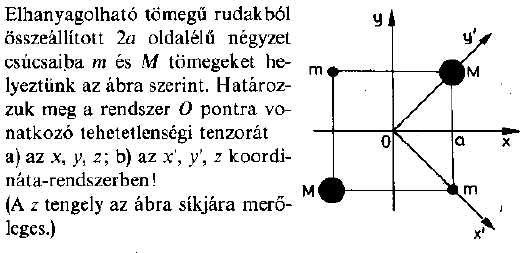
\includegraphics[scale=0.8]{lusta/merev_test1pelda.png}

A c) és d) alfeladatokhoz számold ki az egyik $M$ tömegű testbe helyezett origóra a tehetetlenségi nyomaték tenzort az a) és a b) esetekben párhuzamos tengelyekre!
\paragraph{Megoldás}
Az a) esetben, az 1, jobb felső síknegyedből indulva az egyes testek koordinátái rendre
\[\begin{aligned}
  {{\mathbf{r}}_1} =  & a\left( {\phantom{-}1,\phantom{-}1,0} \right), \\ 
  {{\mathbf{r}}_2} =  & a\left( {\phantom{-}1, - 1,0} \right), \\ 
  {{\mathbf{r}}_3} =  & a\left( { - 1, - 1,0} \right) \text{ és} \\ 
  {{\mathbf{r}}_4} =  & a\left( {\phantom{-}1, - 1,0} \right). \\ 
\end{aligned} \]
A ${\mathbf{\Theta }}$ bármelyik helyén megjelenő koordináta $z$ komponense 0, így kiemelve $a$-t kapjuk, hogy 
\[\begin{aligned}
  {\mathbf{\Theta }} &  = {a^2}\left( {\begin{array}{*{20}{c}}
  {\sum\limits_i {{m_i}{{\left( {{y_i}/a} \right)}^2}} }&{ - \sum\limits_i {{m_i}\left( {{x_i}/a} \right)\left( {{y_i}/a} \right)} }&0 \\ 
  {{\Theta _{12}}}&{\sum\limits_i {{m_i}{{\left( {{x_i}/a} \right)}^2}} }&0 \\ 
  0&0&{{\Theta _{11}} + {\Theta _{22}}} 
\end{array}} \right) \\ 
   &  = {a^2}\left( {\begin{array}{*{20}{c}}
  {M + m + M + m}&{ - M + m - M + m}&0 \\ 
  {{\Theta _{12}}}&{M + m + M + m}&0 \\ 
  0&0&{{\Theta _{11}} + {\Theta _{22}}} 
\end{array}} \right) \\ 
   &  = 2{a^2}\left( {\begin{array}{*{20}{c}}
  {M + m}&{m - M}&0 \\ 
  {m - M}&{M + m}&0 \\ 
  0&0&{2\left( {M + m} \right)} 
\end{array}} \right). \\ 
\end{aligned} \]

A b), c) és d) alrészek házi feladatok, a megoldások órán lesznek ismertetve. A házi feladatok a továbbiakban a feladatlapon találhatóak.

\subsubsection{Integrális rúd}
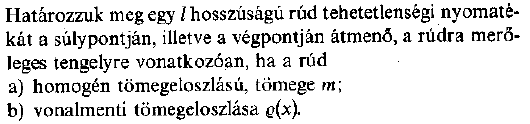
\includegraphics[scale=0.8]{lusta/merev_test2pelda.png} 

A rúd elég vékony, a hossztengelye mentén egy szakasszal modellezhető ebben a feladatban. Ez a feladat házi feladat, a megoldások órán lesznek ismertetve.

\section{Rugalmas szilárd testek}
\subsection{Bemelegítés}
\[\Delta l = \frac{1}{E} \cdot l\frac{F}{A} \Leftrightarrow \left\{ \begin{aligned}
  \frac{{\Delta l}}{l}E =  & \frac{F}{A} \\ 
  \varepsilon E =  & \sigma  \\ 
\end{aligned}  \right.\]
Előadáson szerepelt, hogy az anyagok Young-modulusza nagyságrendileg $E = 100{\text{ GPa}}$. Mennyivel lesz hosszabb egy $1{\text{ m}}$ hosszúságú, $1{\text{ mm}}$ átmérőjű bronz drót, amire földi körülmények között $1{\text{ kg}}$-nyi súlyt akasztunk, ha a Young-modulusza éppen $100{\text{ GPa}}$ és sűrűsége $\varrho  = 8 \cdot {10^3}{\text{ kg/}}{{\text{m}}^{\text{3}}}$? Mekkora ekkor a relatív megnyúlása? Mekkora ekkor a drótban a feszültség? 

Ha a bronz drótot saját súlyánál fogva lógatjuk fel, milyen hosszú és vastag drótot kell venni, hogy a relatív megnyúlása valahol már elérje az 1 ezreléket? Hol lesz ez a pont? Mekkora lesz ekkor a belső feszültség abban a pontban?

\paragraph{Megoldás}
\[\Delta l = \frac{1}{{100{\text{ GPa}}}}1{\text{ m}}\frac{{1{\text{ kg}} \cdot \overbrace {10{\text{ m}}/{{\text{s}}^2}}^g}}{{\underbrace {\pi {{\left( {\frac{{1{\text{ mm}}}}{2}} \right)}^2}}_{A = {r^2}\pi  = {{\left( {d/2} \right)}^2}\pi }}} = 0{,}13{\text{ mm}}\]
Tehát kicsivel több, mint $0,1\text{ mm}$ lesz a megnyúlása a drótnak. A kezdeti hosszához képest ez az érték, vagyis a relatív megnyúlás egy kicsit több, mint 1 tízezredék. A feszültség ekkor
\[\sigma  = 0,12 \cdot {10^{ - 3}} \cdot 100{\text{ GPa}} = 12{\text{ MPa}}.\]

A drót vastagsága állandó, ezért $\sigma $ magasságfüggése csak az erő magasságfüggésén keresztül jön be, $\sigma \left( h \right) = F\left( h \right)/A$. Egy adott pontban ható erő a pont alatt lévő drót teljes tömegétől függ, amely a felfüggesztési pontban nézve maximális. Erre a pontra felírva: 

\[\begin{aligned}
  0{,}001 = \varepsilon  = \frac{1}{E}\sigma  =  & \frac{1}{E}\frac{F}{A} \\ 
   =  & \frac{1}{E}\frac{{\overbrace {\overbrace {A \cdot l}^V \varrho }^m \cdot g}}{A} \\ 
   =  & \frac{1}{E}\varrho  \cdot l \cdot g \Rightarrow l = \frac{{\varepsilon E}}{{\varrho g}} = \frac{{0,001 \cdot 100{\text{ GPa}}}}{{8 \cdot {{10}^3}{\text{ kg}}/{{\text{m}}^3} \cdot 10{\text{ m}}/{{\text{s}}^2}}} = 1{,}2{\text{ km.}} \\ 
\end{aligned} \]

\subsection{Disztorzió és deformációs gradiens}
Legyenek a referencia-mintánk vektorai vesszőtlenek, a transzformált testté pedig a vesszősek! Mutasson a referencia-mintában két elég közeli helyre az ${{\mathbf{r}}_1}$ és ${{\mathbf{r}}_2}$ vektor\footnote{Ezeknek a vektoroknak olyan értelemben kell közel lenniük, hogy azokat összekösse olyan görbe, amely végig az anyagban halad. Pl.\ egy nyújtatlan, szoros tekercselésű rugó szomszédos menetei hiába érintkeznek, nem vehetem az egyik vektort az egyik, a másik vektort a másik menetből.}! A transzformációt hatására ezek rendre ${\mathbf{r}}_1'$ és ${\mathbf{r}}_2'$ vektorokba mennek át, általánosan \[{\mathbf{r}}' = {\mathbf{r}} + {\mathbf{u}}\left( {\mathbf{r}} \right).\]
Vezessük még be az alábbi jelöléseket:
\[\begin{gathered}
  \Delta {\mathbf{r}} = {{\mathbf{r}}_2} - {{\mathbf{r}}_1}, \hfill \\
  \Delta {\mathbf{r}}' = {{\mathbf{r}}_2'} - {{\mathbf{r}}_1'}. \hfill \\ 
\end{gathered} \]
A jelölések áttekintéséhez tekintsük \aref{fig:u}. ábrát!
\begin{figure}[htb] 
\centering    
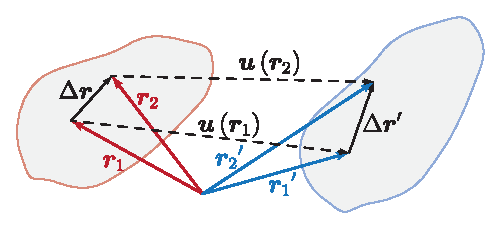
\includegraphics[scale=1]{figs/u.eps}
\caption{Az ${\mathbf{u}}\left( {\mathbf{r}} \right)$ elmozdulásmező szemléltetése: bal oldalt a nyújtatlan, eredeti testünk a vesszőtlen vektorokkal, jobbra a nyújtott és esetleg (párhuzamos eltolással és forgatással) eltolt test a vesszős koordinátákkal.}
\label{fig:u}
\end{figure}
\FloatBarrier

Ekkor az ábráról leolvasható módon:
\begin{align} \label{eq:kul_vektor}
  \underbrace {{{\mathbf{r}}_2}' - {{\mathbf{r}}_1}'}_{\Delta {\mathbf{r}}'} =  & {\mathbf{u}}\left( {{{\mathbf{r}}_2}} \right) + \underbrace {{{\mathbf{r}}_2} - {{\mathbf{r}}_1}}_{\Delta {\mathbf{r}}} - {\mathbf{u}}\left( {{{\mathbf{r}}_1}} \right) \nonumber \\ 
  \Delta {\mathbf{r}}' =  & \Delta {\mathbf{r}} + {\mathbf{u}}\left( {{{\mathbf{r}}_1} + \Delta {\mathbf{r}}} \right) - {\mathbf{u}}\left( {{{\mathbf{r}}_1}} \right),
\end{align}
így ha ${\Delta {\mathbf{r}}}$ elég kicsi, akkor írhatjuk ezt úgy, hogy 
\begin{equation} \label{eq:disztrozio_def}
\Delta {\mathbf{r}}' = \Delta {\mathbf{r}} + {\left. {\frac{{d{\mathbf{u}}\left( {\mathbf{r}} \right)}}{{d{\mathbf{r}}}}} \right|_{{{\mathbf{r}}_1}}} \cdot \Delta {\mathbf{r}} = \underbrace {\left( {{\mathbf{I}} + {{\left. {{{\mathbf{\beta }}^T}} \right|}_{{{\mathbf{r}}_1}}}} \right)}_{\mathbf{F}}\Delta {\mathbf{r}},
\end{equation}
ahol a bevezetett ${\mathbf{\beta }}$ a \textbf{disztorzió}, és ezen \eqref{eq:disztrozio_def}.\ képlet szerint a definíciója:
\begin{equation} \label{eq:disztrozio_szamolas}
{\beta _{ij}} = {\partial _i}{u_j} \Leftrightarrow {{\mathbf{\beta }}^T}\left( {\mathbf{r}} \right) = \frac{{d{\mathbf{u}}}}{{d{\mathbf{r}}}},
\end{equation}
valamint bevezethetjük még a \textbf{deformációs gradienst}, amelyre
\[\begin{aligned}
  {\mathbf{F}}\left( {\mathbf{r}} \right) &  = \frac{d}{{d{\mathbf{r}}}}{\mathbf{r}}' \\ 
   &  = \frac{d}{{d{\mathbf{r}}}}\left( {{\mathbf{r}} + {\mathbf{u}}\left( {\mathbf{r}} \right)} \right) \\ 
   &  = {\mathbf{I}} + {{\mathbf{\beta }}^T}\left( {\mathbf{r}} \right). \\ 
\end{aligned} \]

Néha előfordul, hogy a deformációs gradiens térben állandó. Ekkor igaz lesz, hogy ${\mathbf{r}}' = {\mathbf{Fr}}$, mert ennek deriváltjaként épp megkapjuk ${\mathbf{F}}$-et.

\subsection{Deformáció}
Fejezzük ki az anyagban két pont távolságának a megváltozását, azaz $\left| {\Delta {\mathbf{r}}'} \right| - \left| {\Delta {\mathbf{r}}} \right|$ mennyiséget! Ehhez először fejezzük ki ${\left| {\Delta {\mathbf{r}}'} \right|^2}$-et:
\[\begin{aligned}
  {\left| {\Delta {\mathbf{r}}'} \right|^2} =  & \Delta {\mathbf{r}}' \cdot \Delta {\mathbf{r}}' \\ 
   =  & \left( {{\mathbf{I}} + {{\mathbf{\beta }}^T}} \right)\Delta {\mathbf{r}} \cdot \left( {{\mathbf{I}} + {{\mathbf{\beta }}^T}} \right)\Delta {\mathbf{r}} \\ 
   =  & \Delta {\mathbf{r}}^T\underbrace {\left( {{\mathbf{I}} + {\mathbf{\beta }}} \right)\left( {{\mathbf{I}} + {{\mathbf{\beta }}^T}} \right)}_{\left( {{\mathbf{I}} + {\mathbf{\beta }} + {{\mathbf{\beta }}^T} + {\mathbf{\beta }}{{\mathbf{\beta }}^T}} \right)}\Delta {\mathbf{r}} \\ 
   =  & {\left( {\Delta {\mathbf{r}}} \right)^2} + \Delta {\mathbf{r}}^T\left( {{\mathbf{\beta }} + {{\mathbf{\beta }}^T} + {\mathbf{\beta }}{{\mathbf{\beta }}^T}} \right)\Delta {\mathbf{r}} .\\ 
\end{aligned} \]
Ebből
\begin{align} \label{eq:deform_def}
  \left| {\Delta {\mathbf{r}}'} \right| =  & \left| {\Delta {\mathbf{r}}} \right|\sqrt {1 + \frac{{\Delta {\mathbf{r}}^T}}{{\left| {\Delta {\mathbf{r}}} \right|}}\left( {{\mathbf{\beta }} + {{\mathbf{\beta }}^T} + {\mathbf{\beta }}{{\mathbf{\beta }}^T}} \right)\frac{{\Delta {\mathbf{r}}}}{{\left| {\Delta {\mathbf{r}}} \right|}}}  \nonumber \\ 
   =  & \left| {\Delta {\mathbf{r}}} \right|\sqrt {1 + {{\mathbf{e}}_{\Delta {\mathbf{r}}}^T}2{\mathbf{\varepsilon }}{{\mathbf{e}}_{\Delta {\mathbf{r}}}}},
\end{align}
ahol bevezettük az ${\Delta {\mathbf{r}}}$ irányú egységvektort, ${{\mathbf{e}}_{\Delta {\mathbf{r}}}}$-t, illetve a deformációs tenzort,
\[\begin{aligned}
  2{\mathbf{\varepsilon }}\left( {\mathbf{r}} \right) &  = {\mathbf{\beta }}\left( {\mathbf{r}} \right) + {{\mathbf{\beta }}^T}\left( {\mathbf{r}} \right) + {\mathbf{\beta }}\left( {\mathbf{r}} \right){{\mathbf{\beta }}^T}\left( {\mathbf{r}} \right) \\ 
  {\mathbf{\varepsilon }}\left( {\mathbf{r}} \right) &  = \frac{{{\mathbf{\beta }}\left( {\mathbf{r}} \right) + {{\mathbf{\beta }}^T}\left( {\mathbf{r}} \right)}}{2} + \frac{{{\mathbf{\beta }}\left( {\mathbf{r}} \right){{\mathbf{\beta }}^T}\left( {\mathbf{r}} \right)}}{2} \\ 
   &  = {{\mathbf{\beta }}^{{\text{sz}}}}\left( {\mathbf{r}} \right) + \frac{{{\mathbf{\beta }}\left( {\mathbf{r}} \right){{\mathbf{\beta }}^T}\left( {\mathbf{r}} \right)}}{2}.\\ 
\end{aligned} \]

Itt bevezettük a mátrix szimmetrikus részének a definícióját, ami \aref{sec:kicsi_def}.\ pontban található. Megjegyzendő még, hogy amennyiben egy deformáció kicsi, úgy a második tag, a disztorzióban másodrendű tag elhanyagolhatóvá válik.

\subsection{Relatív térfogatváltozás}
Nézzük meg, hogyan változik meg egy $V$ nagyságú térfogatelem, amelyet a
\[{\mathbf{x}} = \left( {\begin{array}{*{20}{c}}
  1 \\ 
  0 \\ 
  0 
\end{array}} \right)x,\quad {\mathbf{y}} = \left( {\begin{array}{*{20}{c}}
  0 \\ 
  1 \\ 
  0 
\end{array}} \right)y,\quad {\mathbf{z}} = \left( {\begin{array}{*{20}{c}}
  0 \\ 
  0 \\ 
  1 
\end{array}} \right)z\]
vektorok kijelölnek! Ez könnyedén kifejezhető a három vektor vegyesszorzatával, azaz
\[V = \left( {{\mathbf{x}},{\mathbf{y}},{\mathbf{z}}} \right) = \left| {\begin{array}{*{20}{c}}
  x&0&0 \\ 
  0&y&0 \\ 
  0&0&z 
\end{array}} \right| = x \cdot y \cdot z.\]

Ha ${\mathbf{F}}$ nem lenne konstans, akkor legyenek ezek a vektorok elég kicsik abban az értelemben, hogy ${\mathbf{F}}$ már konstansnak tekinthető a vektorok által kijelölt térfogatban. \Aref{eq:kul_vektor}.\ egyenletben lévő $\Delta$-kat mániákusan kiírva, de fejben tartva, hogy a különbségvektorokat az origó nullváktorával képezzük, \aref{eq:disztrozio_def}.\ egyenletet így írhatjuk a három vektorra:
\[\begin{aligned}
  \Delta {\mathbf{x}}' =  & \Delta {\mathbf{x}} + {\mathbf{u}}\left( {\mathbf{x}} \right) - {\mathbf{u}}\left( 0 \right) = \underbrace {\left( {{\mathbf{I}} + \frac{{d{\mathbf{u}}}}{{d{\mathbf{r}}}}} \right)}_{{\mathbf{F}} = {\text{konstans}}}\Delta {\mathbf{x}} \\ 
  \Delta {\mathbf{y}}' =  & \Delta {\mathbf{y}} + {\mathbf{u}}\left( {\mathbf{y}} \right) - {\mathbf{u}}\left( 0 \right) = \left( {{\mathbf{I}} + \frac{{d{\mathbf{u}}}}{{d{\mathbf{r}}}}} \right)\Delta {\mathbf{y}} \\ 
  \Delta {\mathbf{z}}' =  & \Delta {\mathbf{z}} + {\mathbf{u}}\left( {\mathbf{z}} \right) - {\mathbf{u}}\left( 0 \right) = \left( {{\mathbf{I}} + \frac{{d{\mathbf{u}}}}{{d{\mathbf{r}}}}} \right)\Delta {\mathbf{z}}. \\ 
\end{aligned} \]
Ekkor a transzformáció után a vektorok alakja:
\[{\mathbf{x}}' = \left( {\begin{array}{*{20}{c}}
  {1 + {\partial _x}{u_x}} \\ 
  {{\partial _x}{u_y}} \\ 
  {{\partial _x}{u_z}} 
\end{array}} \right)x,\quad {\mathbf{y}}' = \left( {\begin{array}{*{20}{c}}
  {{\partial _y}{u_x}} \\ 
  {1 + {\partial _y}{u_y}} \\ 
  {{\partial _y}{u_z}} 
\end{array}} \right)y,\quad {\mathbf{z}}' = \left( {\begin{array}{*{20}{c}}
  {{\partial _z}{u_x}} \\ 
  {{\partial _z}{u_y}} \\ 
  {1 + {\partial _z}{u_z}} 
\end{array}} \right)z,\]
az új térfogatra pedig
\begin{equation*}
  V' = \left( {{\mathbf{x}}',{\mathbf{y}}',{\mathbf{z}}'} \right) = \left| {\begin{array}{*{20}{c}}
  {1 + {\partial _x}{u_x}}&{{\partial _x}{u_y}}&{{\partial _x}{u_z}} \\ 
  {{\partial _y}{u_x}}&{1 + {\partial _y}{u_y}}&{{\partial _y}{u_z}} \\ 
  {{\partial _z}{u_x}}&{{\partial _z}{u_y}}&{1 + {\partial _z}{u_z}} 
\end{array}} \right| x y z  = \det \left( {\mathbf{F}} \right)V. 
\end{equation*}
Az új térfogat a régihez viszonyítva, illetve a relatív térfogatváltozásra kapjuk, hogy
\begin{equation} \label{eq:rel_terfogatv}
\frac{{V'}}{V} = \det \left( {\mathbf{F}} \right) \Leftrightarrow \frac{{V' - V}}{V} = \frac{{\Delta V}}{V} = \det \underbrace {\left( {{\mathbf{I}} + {\mathbf{\beta^T }}} \right)}_{\mathbf{F}} - 1.
\end{equation}

Infinitezimális deformáció esetét \aref{sec:kicsi_def}.\ fejezet tárgyalja.

\subsection{Kicsi deformációk} \label{sec:kicsi_def}
Nagy jelentősége van annak a határesetnek, amikor a transzformáció kicsi, mert ekkor a testben ébredő belső feszültségek a deformációval arányosak lesznek (a lineáris rugalmasságtan általánosított Hooke-törvénye). Továbbá gyakran könnyebb is az ebben az esetben kapott mennyiségekkel (deformációval, relatív térfogatváltozással) számolni, illetve elég kicsi időre nézve a transzformációk is elég kicsik. Milyen egyszerűbb formálkhoz juthatunk tehát a kis transzformációk esetén?

Ha a disztorzió kicsi, akkor a deformáció \told\aref{eq:deform_def}+as{} egyenlet szerinti definíciójában elhanyagolható a ${\mathbf{\beta }}\left( {\mathbf{r}} \right){{\mathbf{\beta }}^T}\left( {\mathbf{r}} \right)$ tag a ${\mathbf{\beta}}\left( {\mathbf{r}} \right)$-hoz és ${\mathbf{\beta^T}}\left( {\mathbf{r}} \right)$-hoz képest, és 
\begin{equation}
{\mathbf{\varepsilon }}\left( {\mathbf{r}} \right) = \frac{{{\mathbf{\beta }}\left( {\mathbf{r}} \right) + {{\mathbf{\beta }}^T}\left( {\mathbf{r}} \right)}}{2}.
\end{equation}
Viszont ekkor ${\mathbf{\varepsilon }}$ is kicsi, így \az{\eqref{eq:deform_def}} egyenletben a gyököt 1 körül sorfejtve kapjuk, hogy
\[\left| {\Delta {\mathbf{r}}'} \right| = \left| {\Delta {\mathbf{r}}} \right|\left( {1 + \frac{{{{\mathbf{e}}_{\Delta {\mathbf{r}}}}2{\mathbf{\varepsilon }}{{\mathbf{e}}_{\Delta {\mathbf{r}}}}}}{2}} \right) \Rightarrow \frac{{\left| {\Delta {\mathbf{r}}'} \right|}}{{\left| {\Delta {\mathbf{r}}} \right|}} - 1 = {{\mathbf{e}}_{\Delta {\mathbf{r}}}}{\mathbf{\varepsilon }}{{\mathbf{e}}_{\Delta {\mathbf{r}}}}.\]

Itt megjelent a ${\Delta {\mathbf{r}}}$ irányú relatív hosszváltozás. Fontos, hogy ez a formula csak akkor igaz, ha a disztorzió kicsi volt. Ez nem csak, hogy egyszerűbb alakra hozta a deformációt a disztorzió függvényeként, de a relatív hosszváltozás is egyszerűbben kifejezhetővé vált.

\paragraph{Szimmetrikus és antiszimmetrikus részekre} bonthatunk egy operátor az alábbi definíció szerint:
\[{{\mathbf{A}}^{{\text{sz}}}} = \frac{{{\mathbf{A}} + {{\mathbf{A}}^T}}}{2}\quad {{\mathbf{A}}^{\text{asz}}} = \frac{{{\mathbf{A}} - {{\mathbf{A}}^T}}}{2},\]
ahol a $T$ felső index a transzponálást jelenti. Ekkor minden operátor felírható ezek összegeként,
\[{\mathbf{A}} = {{\mathbf{A}}^{{\text{sz}}}} + {{\mathbf{A}}^{{\text{asz}}}},\]
valamint igaz erre a felbontásra, hogy \[{\left( {{{\mathbf{A}}^{{\text{sz}}}}} \right)^T} = {{\mathbf{A}}^{\text{sz}}}\quad {\left( {{{\mathbf{A}}^{{\text{asz}}}}} \right)^T} =  - {{\mathbf{A}}^{{\text{asz}}}}.\]
Ennek szellemében kicsi deformációt a disztorziónak csak a szimmetrikus része okoz,
\[{\mathbf{\varepsilon }}\left( {\mathbf{r}} \right) = {{\mathbf{\beta }}^{{\text{sz}}}}\left( {\mathbf{r}} \right).\]
Nincs tehát bijekció a deformáció és a disztorzió között. A disztorzióból kiszámolható a deformáció, de a deformációból a disztorzió nem, csak annak szimmetrikus része adható meg. Ez azt is jelenti, hogy tisztán antiszimmetrikus disztorzió nem hoz létre deformációt. A tisztán antiszimmetrikus, infinitezimális disztrozió forgatást ír le, ahogy azt \aref{section:forgatas} fejezetben, az infinitezimális forgatásnál látni fogjuk.

További azonosság még, hogy \[\begin{aligned}
  {\text{Tr}}\left( {\mathbf{\beta }} \right) =  & {\text{Tr}}\left( {{{\mathbf{\beta }}^{{\text{sz}}}} + {{\mathbf{\beta }}^{{\text{asz}}}}} \right) \\ 
   =  & {\text{Tr}}\left( {{{\mathbf{\beta }}^{{\text{sz}}}}} \right) + \underbrace {{\text{Tr}}\left( {{{\mathbf{\beta }}^{{\text{asz}}}}} \right)}_0 \\ 
   =  & {\text{Tr}}\left( {{{\mathbf{\beta }}^{{\text{sz}}}}} \right), \\ 
\end{aligned} \] így kicsi disztorziókra $Tr\left( {\mathbf{\beta }} \right) = Tr\left( {\mathbf{\varepsilon }} \right)$. Ez az összefüggés jól jön a relatív térfogatváltozás számolásánál \aref{section:rel_volume} pontban.



\subsubsection{Relatív térfogatváltozás} \label{section:rel_volume}

Gyakori eset, hogy a disztorzióban a deriváltak az $1$-hez képest kicsik, így a relatív térfogatváltozás \ref{eq:rel_terfogatv}.\ egyenletében elsőrendig megtartva a $\det \left( {\mathbf{F}} \right)$ tagjait, a másod- és magasabbrendű tagokat pedig elhanyagolva kapjuk, hogy 
\[\begin{aligned}
  V' \approx  & \left( {1 + {\partial _x}{u_x}} \right)\left( {1 + {\partial _y}{u_y}} \right)\left( {1 + {\partial _z}{u_z}} \right) \cdot V \\ 
   \approx  & \left( {1 + {\partial _x}{u_x} + {\partial _y}{u_y} + {\partial _z}{u_z}} \right) \cdot V =  \\ 
   =  & \left( {1 + {\text{Tr}}\left( {\mathbf{\beta }} \right)} \right) \cdot V\quad \quad {\text{Tr}}\left( {\mathbf{\beta }} \right) = {\text{Tr}}\left( {{{\mathbf{\beta }}^{{\text{sz}}}}} \right) = {\text{Tr}}\left( {{{\mathbf{\varepsilon }}}} \right) \\ 
   =  & \left( {1 + {\text{Tr}}\left( {{\mathbf{\varepsilon }}} \right)} \right) \cdot V \\ 
\end{aligned} \]
ahol megjelent a deformációs tenzor trace-e, avagy spúrja, amit a ${\text {Tr}}$ vagy ${\text {Sp}}$ operátor jelöl, ami megadja a főátlóbeli elemek összegét. Ekkor a relatív térfogatváltozás egyszerűen a deformációs tenzor trace-e, azaz
\[\frac{{V' - V}}{V} = \frac{{\Delta V}}{V} = {\text{Tr}}\left( {\mathbf{\varepsilon }} \right).\]

\subsection{Egyszerű transzformációk}
\subsubsection{Eltolás}
Eltolásnál minden helyvektorhoz egy ${{\mathbf{r}}_0}$ helyvektort adunk, amelyet \az{\ref{fig:eltolas}}.\ ábra szemléltet. 
\begin{figure}[htb] 
\centering    
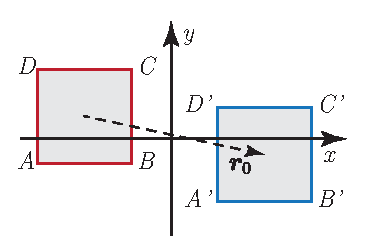
\includegraphics[scale=1]{figs/eltolas.eps}
\caption{Az eltolás szemléltetése.}
\label{fig:eltolas}
\end{figure}
\FloatBarrier
Ekkor az új vektorokra és az elmozdulástérre
\[\begin{aligned}
  {\mathbf{r}}'\left( {\mathbf{r}} \right) &  = {\mathbf{r}} + {{\mathbf{r}}_0}, \\ 
  {\mathbf{u}}\left( {\mathbf{r}} \right) &  = {{\mathbf{r}}_0}, \\ 
\end{aligned} \]
a disztorziót pedig számolhatjuk egyből ${\mathbf{u}}$ deriváltjából, vagy leolvashatjuk a $\Delta {\mathbf{r}}'$ értékéből,
\[\Delta {{\mathbf{r}}^\prime } = {{\mathbf{r}}_2}^\prime  - {{\mathbf{r}}_1}^\prime  = \left( {{{\mathbf{r}}_2} + {{\mathbf{r}}_0}} \right) - \left( {{{\mathbf{r}}_1} + {{\mathbf{r}}_0}} \right) = \Delta {\mathbf{r}} = \left( {{\mathbf{I}} + {\mathbf{0}}} \right)\Delta {\mathbf{r}} \Rightarrow \left\{ {\begin{array}{*{20}{c}}
  {{{\mathbf{\beta }}^T} = {\mathbf{0}}} \\ 
  {{\mathbf{F}} = {\mathbf{I}}} 
\end{array}} \right..\]
Triviálisan látszik, hogy a deformációra ${\mathbf{\varepsilon}} = {\mathbf{0}}$.

\footnotesize
\paragraph{Példa}
Legyen a testünk $A$ és $B$ pontjainak koordinátái ${{\mathbf{r}}_A} = \left( { - 3, - 0.5, 0} \right)$ és ${{\mathbf{r}}_B} = \left( { - 0.5, - 0.5, 0} \right)$, valamint $\Delta {\mathbf{r}} = {{\mathbf{r}}_B} - {{\mathbf{r}}_A}$! Legyen az elmozdulásmező a térben helytől független állandó, ${\mathbf{u}}\left( {\mathbf{r}} \right) = \left( {2, - 1} \right)$. 
Mire módosul a transzformáció után a $\Delta {\mathbf{r}}$ vektor? Mennyi ekkor a disztorzió és a deformációs gradiens?

\textbf{Megoldás:} Felírva az új koordinátákat, illetve a különbségvektort (a $z$ koordináta, és az abban vett különbségek mindig 0-k):
\[\begin{gathered}
  {{\mathbf{r}}_A}' = {{\mathbf{r}}_A} + {\mathbf{u}} = \left( { - 3, - 0.5} \right) + \left( {2, - 1} \right) = \left( { - 1, - 1.5} \right), \hfill \\
  {{\mathbf{r}}_B}' = {{\mathbf{r}}_B} + {\mathbf{u}} = \left( { - 0.5, - 0.5} \right) + \left( {2, - 1} \right) = \left( {1.5, - 1.5} \right), \hfill \\
  \Delta {\mathbf{r}} = {{\mathbf{r}}_B} - {{\mathbf{r}}_A} = \left( { - 0.5, - 0.5} \right) - \left( { - 3, - 0.5} \right) = \left( {2.5,0} \right), \hfill \\
  \Delta {\mathbf{r}}' = {{\mathbf{r}}_B}' - {{\mathbf{r}}_A}' = \left( {1.5, - 1.5} \right) - \left( { - 1, - 1.5} \right) = \left( {2.5,0} \right). \hfill \\ 
\end{gathered} \]
Felírva a definícióját a disztorziónak:
\[{{\mathbf{\beta }}^T}\left( {\mathbf{r}} \right) = \frac{{d{\mathbf{u}}}}{{d{\mathbf{r}}}} = 0.\]
Ebből a deformációs gradiens \[{\mathbf{F}} = {\mathbf{I}} + {{\mathbf{\beta }}^T} = {\mathbf{I}}.\] Ez utóbbit abból is láthattuk volna most, hogy ${\mathbf{F}}$-et a $\Delta {\mathbf{r}}' = {\mathbf{F}}\Delta {\mathbf{r}}$ összefüggés adja meg, és most fenn állt a $\Delta {\mathbf{r}}' = \Delta {\mathbf{r}}$ összefüggés.
\normalsize

\subsubsection{Nyújtás}
Nyújtásnál minden régi helyvektort (megfelelő koordináta rendszerben) komponensenként egy számmal szorzunk, amelyet \az{\ref{fig:nyujtas}}.\ ábra szemléltet. Ekkor
\begin{multline*}
{\mathbf{r}}'\left( {\mathbf{r}} \right) = \left( {\begin{array}{*{20}{c}}
  {x'} \\ 
  {y'} \\ 
  {z'} 
\end{array}} \right) = \left( {\begin{array}{*{20}{c}}
  {{\lambda _1}x} \\ 
  {{\lambda _2}y} \\ 
  {{\lambda _3}z} 
\end{array}} \right) = \left( {\begin{array}{*{20}{c}}
  {{\lambda _1}}&0&0 \\ 
  0&{{\lambda _2}}&0 \\ 
  0&0&{{\lambda _3}} 
\end{array}} \right)\left( {\begin{array}{*{20}{c}}
  x \\ 
  y \\ 
  z 
\end{array}} \right) = \\ = \left[ {{\lambda _1}\left( {{{\mathbf{e}}_1} \circ {{\mathbf{e}}_1}} \right) + {\lambda _2}\left( {{{\mathbf{e}}_2} \circ {{\mathbf{e}}_2}} \right) + {\lambda _3}\left( {{{\mathbf{e}}_3} \circ {{\mathbf{e}}_3}} \right)} \right]{\mathbf{r}},
\end{multline*}
amelyben ${\lambda _i} \in \mathbb{R}$.

Ekkor az elmozdulástér
\[{\mathbf{u}}\left( {\mathbf{r}} \right) = {\mathbf{r}}' - {\mathbf{r}} = \underbrace {\left( {\begin{array}{*{20}{c}}
  {{\lambda _1}}&0&0 \\ 
  0&{{\lambda _2}}&0 \\ 
  0&0&{{\lambda _3}} 
\end{array}} \right)}_{\mathbf{\lambda }}{\mathbf{r}} - {\mathbf{r}} = \left( {{\mathbf{\lambda }} - {\mathbf{I}}} \right){\mathbf{r}} = \left( {\begin{array}{*{20}{c}}
  {{\lambda _1} - 1}&0&0 \\ 
  0&{{\lambda _2} - 1}&0 \\ 
  0&0&{{\lambda _3} - 1} 
\end{array}} \right){\mathbf{r}},\]
amelyből deriválással megkapható a disztorzió, vagy kifejezhetjük $\Delta {\mathbf{r}}'$-t is,
\[\Delta {\mathbf{r}}' = {{\mathbf{r}}_2}' - {{\mathbf{r}}_1}' = {\mathbf{\lambda }}{{\mathbf{r}}_2} - {\mathbf{\lambda }}{{\mathbf{r}}_1} = {\mathbf{\lambda }}\Delta {\mathbf{r}} = \underbrace {\left( {{\mathbf{I}} + \left( {{\mathbf{\lambda }} - {\mathbf{I}}} \right)} \right)}_{{\mathbf{F}} = {\mathbf{I}} + {{\mathbf{\beta }}^T}}\Delta {\mathbf{r}}\]
amelyből egyszerűen leolvasható a disztorzió és a deformációs gradiens. 

Egy speciális eset az, amikor a mátrix minden koordinátarendszerben diagonális, ez pedig az egységoperátor konstansszorosa. Ha a nyújtás iránytól független, azaz izotróp, akkor ${\lambda _1} = {\lambda _2} = {\lambda _3}$, ekkor az ${\mathbf{I}}$ egységoperátorral
\[{\mathbf{r}}'\left( {\mathbf{r}} \right) = {\lambda _1}{\mathbf{r}} = {\lambda _1}{\mathbf{Ir}}.\]

Minden szimmetrikus, de nem diagonális, térben konstans deformációs gradiens nyújtást ír le, mert a szimmetrikus mátrixok diagonalizálhatók. Egy speciális eset a tiszta nyírás (lásd \ref{sec:tiszta_nyiras}), amikor a deformációs gradiens mátrix determinánsa 1 (vagy éppen $-1$, ha megengedjük).

Másik speciális eset, ha csak egyetlen $\lambda$ értéke nem 1, ekkor a nyújtást egytengelyűnek nevezzük. Belátható, hogy minden nem egytengelyű nyújtás legfeljebb három egytengelyű nyújtás egymásutánjaként is előáll.

\begin{figure}[htb] 
\centering    
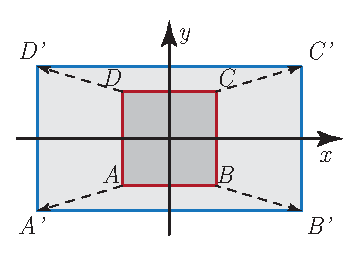
\includegraphics[scale=1]{figs/nyujtas.eps}
\caption{A nyújtás szemléltetése.}
\label{fig:nyujtas}
\end{figure}

\footnotesize
\paragraph{Példa}
Legyen a testünk $A$ és $B$ pontjainak koordinátáira ${{\mathbf{r}}_A} = \left( { - 3, - 0.5, 0} \right)$ és ${{\mathbf{r}}_B} = \left( { - 0.5, - 0.5, 0} \right)$, valamint $\Delta {\mathbf{r}} = {{\mathbf{r}}_B} - {{\mathbf{r}}_A}$! Végezzünk el a testünkön egy transzformációt, amelynek során minden régi ${\mathbf{r}} = \left( {x,y,z} \right)$ helyvektor az alábbi ${\mathbf{r}}' = \left( {x',y',z'} \right)$ helyvektorba megy át: 
\[\begin{aligned}
  x' &  = 2 \cdot x \\ 
  y' &  = 3 \cdot y \\ 
  z' &  = 1 \cdot z. \\ 
\end{aligned} \]

Írd fel az elmozdulásmezőt vektoros alakban! Mire változik a $\Delta {\mathbf{r}}$ vektor? Mennyi a disztorzió, a deformációs gradiens és a relatív térfogatváltozás?

Tegyük át és rögzítsük az origót az anyagon az $A$ ponton és írjuk le innen is a nyújtást! Legyenek a vektoraink a csillagosak, ${{\mathbf{r}}_A}^*$ és ${{\mathbf{r}}_B}^*$. Hogyan változnak transzformációra általánosan a vektorok? Azaz add meg az ${\mathbf{r}}{{^*}'}\left( {{{\mathbf{r}}^ * }} \right)$ függvényt! Mi az elmozdulástér, a disztorzió, a $\Delta {{\mathbf{r}}^ * }'$, a deformációs gradiens és a relatív térfogatváltozás?

\paragraph{Megoldás}
Az új helyvektorok és abból az elmozdulástér:
\[{\mathbf{r}}' = \left( {\begin{array}{*{20}{c}}
  2&0&0 \\ 
  0&3&0 \\ 
  0&0&1 
\end{array}} \right){\mathbf{r}}\quad {\mathbf{r}}' = {\mathbf{r}} + {\mathbf{u}}\left( {\mathbf{r}} \right) \Rightarrow {\mathbf{u}}\left( {\mathbf{r}} \right) = {\mathbf{r}}'\left( {\mathbf{r}} \right) - {\mathbf{r}} = \left( {\begin{array}{*{20}{c}}
  x \\ 
  {2 \cdot y} \\ 
  0 
\end{array}} \right) = \left( {\begin{array}{*{20}{c}}
  1&0&0 \\ 
  0&2&0 \\ 
  0&0&0 
\end{array}} \right){\mathbf{r}}\]

A két új vektor
\[\begin{aligned}
  {{\mathbf{r}}_A}' = \left( {\begin{array}{*{20}{c}}
  2&0&0 \\ 
  0&3&0 \\ 
  0&0&1 
\end{array}} \right)\left( {\begin{array}{*{20}{c}}
  { - 3} \\ 
  { - 0.5} \\ 
  0 
\end{array}} \right) =  - \left( {\begin{array}{*{20}{c}}
  6 \\ 
  {1.5} \\ 
  0 
\end{array}} \right) \\ 
  {{\mathbf{r}}_B}' = \left( {\begin{array}{*{20}{c}}
  2&0&0 \\ 
  0&3&0 \\ 
  0&0&1 
\end{array}} \right)\left( {\begin{array}{*{20}{c}}
  { - 0.5} \\ 
  { - 0.5} \\ 
  0 
\end{array}} \right) =  - \left( {\begin{array}{*{20}{c}}
  2 \\ 
  3 \\ 
  0 
\end{array}} \right)/2 \\ 
\end{aligned} \]

A különbségvektorok
\[\begin{aligned}
  \Delta {\mathbf{r}} &  = \left( {\begin{array}{*{20}{c}}
  { - 0.5} \\ 
  { - 0.5} \\ 
  0 
\end{array}} \right) - \left( {\begin{array}{*{20}{c}}
  { - 3} \\ 
  { - 0.5} \\ 
  0 
\end{array}} \right) = \left( {\begin{array}{*{20}{c}}
  {2.5} \\ 
  0 \\ 
  0 
\end{array}} \right) \\ 
  \Delta {\mathbf{r}}' &  =  - \left( {\begin{array}{*{20}{c}}
  2 \\ 
  3 \\ 
  0 
\end{array}} \right)/2 + \left( {\begin{array}{*{20}{c}}
  6 \\ 
  {1.5} \\ 
  0 
\end{array}} \right) = \left( {\begin{array}{*{20}{c}}
  5 \\ 
  0 \\ 
  0 
\end{array}} \right) \\ 
\end{aligned} \]

A disztorzió
\[{{\mathbf{\beta }}^T} = \frac{{d{\mathbf{u}}}}{{d{\mathbf{r}}}} = \left( {\begin{array}{*{20}{c}}
  1&0&0 \\ 
  0&2&0 \\ 
  0&0&0 
\end{array}} \right) \Rightarrow {\mathbf{\beta }} = {{\mathbf{\beta }}^T}\]

A deformációs gradiens 
\[{\mathbf{F}} = {\mathbf{I}} + {{\mathbf{\beta }}^T} = \left( {\begin{array}{*{20}{c}}
  2&0&0 \\ 
  0&3&0 \\ 
  0&0&1 
\end{array}} \right)\]

A deformáció
\[{\mathbf{\varepsilon }} = \frac{{{\mathbf{\beta }} + {{\mathbf{\beta }}^T}}}{2} + \frac{{{\mathbf{\beta }}{{\mathbf{\beta }}^T}}}{2} = \left( {\begin{array}{*{20}{c}}
  1&0&0 \\ 
  0&2&0 \\ 
  0&0&0 
\end{array}} \right) + \left( {\begin{array}{*{20}{c}}
  1&0&0 \\ 
  0&4&0 \\ 
  0&0&0 
\end{array}} \right)/2 = \left( {\begin{array}{*{20}{c}}
  {3/2}&0&0 \\ 
  0&4&0 \\ 
  0&0&0 
\end{array}} \right)\]

A relatív térfogatváltozás
\[\frac{{\Delta V}}{V} = \det \left( {\mathbf{F}} \right) - 16 - 1 = 5\]

Miután áttettük az origót az $A$ pontra, az új vektorokra
\[{\mathbf{r}}_A^* = 0 = \left( {{\mathbf{r}}_A^ * } \right)'\]
és
\[{\mathbf{r}}_B^ *  = {{\mathbf{r}}_B} - {{\mathbf{r}}_A}\]
általában pedig
\[{{\mathbf{r}}^ * } = {\mathbf{r}} - {{\mathbf{r}}_A}.\]

Az eltranszformált vektorok a csillagos rendszerben:
\[\begin{aligned}
  \left( {\left( {{{\mathbf{r}}^ * }} \right)'} \right)\underbrace {\left( {{{\mathbf{r}}^ * }} \right)}_{{\text{arg}}} &  = \left( {{\mathbf{r}} - {{\mathbf{r}}_A}} \right)'\left( {{{\mathbf{r}}^ * }} \right) \\ 
   &  = {\mathbf{r}}'\underbrace {\left( {{{\mathbf{r}}^ * }} \right)}_{{\text{arg}}} - {{\mathbf{r}}_A}' \\ 
   &  = {\mathbf{r}}{'^ * } \\ 
\end{aligned} \]

A vesszőzést (transzformálást) azért lehet elvégezni tagonként, mert a transzformáció lineáris. Az eredmény szerint pl.\ az új $B$ pontot a csillagos rendszerből úgy adhatjuk meg, ha a csillagtalanból eltranszformáljuk, majd utána ülünk át a csillagosba,
\[\left( {{\mathbf{r}}_B^ * } \right)' = {\left( {{{\mathbf{r}}_B}'} \right)^*} = {{\mathbf{r}}_B}' - {{\mathbf{r}}_A}' = \Delta {\mathbf{r}}'\]

Így a csillagos eltranszformált különbségvektor ugyanaz, mint a csillagtalan eltranszformált,
\[\Delta {{\mathbf{r}}^ * }' = \left( {{\mathbf{r}}_B^ * } \right)' - \left( {{\mathbf{r}}_A^ * } \right)' = \Delta {\mathbf{r}}' - 0 = \Delta {\mathbf{r}}'\]

Az új koordinátákkal az elmozdulástér
\[\begin{aligned}
  {{\mathbf{u}}^ * }\left( {{{\mathbf{r}}^ * }} \right) &  = {{\mathbf{r}}^ * }' - {{\mathbf{r}}^ * } \\ 
   &  = {\left( {{\mathbf{r}}'} \right)^ * } - {\mathbf{r}} + {{\mathbf{r}}_A} \\ 
   &  = {\mathbf{r}}' - {{\mathbf{r}}_A} - {\mathbf{r}} + {{\mathbf{r}}_A} \\ 
   &  = {\mathbf{r}}' - {\mathbf{r}} = {\mathbf{u}}\left( {\mathbf{r}} \right) \\ 
\end{aligned} \]
Ebből pedig tudható, hogy mind a disztorzió, a deformáció, a deformációs gradiens és a relatív térfogatváltozás is ugyanaz lesz, mint eddig. Tehát a nyújtás során nem kell azt gondolni, hogy a testnek a középpontjában vagyunk, mert minden pontból a nyújtás ugyanúgy írható lesz. Más szóval a nyújtásnak nincsen egy kitüntetett középpontja.
\normalsize

\subsubsection{Forgatás} \label{section:forgatas}
Forgatásnál minden régi helyvektor nagysága megmarad, csak az irányuk változik meg. A forgatást jellemezzük a szöggel és a forgatás tengelyének az irányával. Egy $z$ tengelyű, $\alpha$ szögű forgatásra
\[{\mathbf{r}}'\left( {\mathbf{r}} \right) = \left( {\begin{array}{*{20}{c}}
  {\cos \left( \alpha  \right)}&{ - \sin \left( \alpha  \right)}&0 \\ 
  { \sin \left( \alpha  \right)}&{\cos \left( \alpha  \right)}&0 \\ 
  0&0&1 
\end{array}} \right)\left( {\begin{array}{*{20}{c}}
  x \\ 
  y \\ 
  z 
\end{array}} \right) = {{\mathbf{O}}_{z,\alpha }}{\mathbf{r}}.\]
Egyezmény szerint a pozitív szögű forgatás óramutató járásával ellentétes irányt jelent, és a mátrixban az első sorban van a negatív előjel. Ezt \az{\ref{fig:forgat}}.\ ábra szemlélteti. (A $z$ tengely a papír síkjából kifelé jön, így alkotnak a tengelyek jobbsodrású rendszert.) Általánosan számolással megmutatható, hogy akárhány forgatás együttes hatása szintén egyetlen forgatás egy jól megválasztott tengely körül, jól megválasztott szöggel.

\begin{figure}[htb] 
\centering    
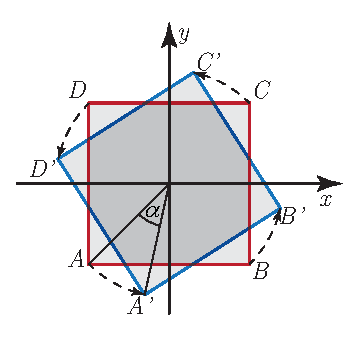
\includegraphics[scale=1]{figs/forgatas.eps}
\caption{A forgatás szemléltetése.}
\label{fig:forgat}
\end{figure}

Az elmozdulástér ekkor:
\[{\mathbf{u}}\left( {\mathbf{r}} \right) = {\mathbf{r}}' - {\mathbf{r}} = {\mathbf{Or}} - {\mathbf{r}} = \left( {{\mathbf{O}} - {\mathbf{I}}} \right){\mathbf{r}}.\]
Ennek deriváltjaként előáll a disztorzió, de megkaphatjuk abból is, ha kiszámoljuk $\Delta {\mathbf{r}}'$-t:
\[\Delta {\mathbf{r}}' = {{\mathbf{r}}_2}' - {{\mathbf{r}}_1}' = {\mathbf{O}}{{\mathbf{r}}_2} - {\mathbf{O}}{{\mathbf{r}}_1} = {\mathbf{O}}\Delta {\mathbf{r}}.\]
Ebből már leolvasható a \textbf{deformációs gradiens} és kiszámolható \textbf{disztorzió}:
\[\begin{aligned}
  {\mathbf{F}} &  = {\mathbf{O}} = {\mathbf{I}} + {{\mathbf{\beta }}^T} \\ 
  {{\mathbf{\beta }}^T} &  = {\mathbf{O}} - {\mathbf{I}}. \\ 
\end{aligned} \]
Megjegyzendő, hogy általános, véges nagyságú forgatásra nem tisztán antiszimmetrikus a disztorzió, annak szimmetrikus komponense is van. A \textbf{deformáció} kiszámolható a disztorzióból, illetve fel kell még használni, hogy a forgatás transzformációja ortogonális (vagyis a transzponáltja az inverze).
\[\begin{aligned}
  2{\mathbf{\varepsilon }} &  = {\mathbf{\beta }} + {{\mathbf{\beta }}^T} + {\mathbf{\beta }}{{\mathbf{\beta }}^T}\quad \quad {{\mathbf{\beta }}^T} = {\mathbf{O}} - {\mathbf{I}} \quad \quad {{\mathbf{\beta }}} = {\mathbf{O}^T} - {\mathbf{I}} \\ 
   &  = {{\mathbf{O}}^T} - {\mathbf{I}} + {\mathbf{O}} - {\mathbf{I}} + \left( {{{\mathbf{O}}^T} - {\mathbf{I}}} \right)\left( {{\mathbf{O}} - {\mathbf{I}}} \right) \\ 
   &  = {{\mathbf{O}}^T} - {\mathbf{I}} + {\mathbf{O}} - {\mathbf{I}} + {{\mathbf{O}}^T}{\mathbf{O}} - {\mathbf{O}} - {{\mathbf{O}}^T} + {\mathbf{I}} \\ 
   &  =  - {\mathbf{I}} + {{\mathbf{O}}^T}{\mathbf{O}}\quad \quad {{\mathbf{O}}^T}{\mathbf{O}} = {\mathbf{I}} \\ 
   &  = 0 \\ 
\end{aligned} \]

\paragraph{Infinitezimális forgatás}
Ha a $z$ tengelyű forgatás kicsi, akkor az új vektorok értékeire
\[\begin{aligned}
  {\mathbf{r}}'\left( {\mathbf{r}} \right) &  = \left( {\begin{array}{*{20}{c}}
  {\cos \left( {\Delta \varphi } \right)}&{ - \sin \left( {\Delta \varphi } \right)}&0 \\ 
  {\sin \left( {\Delta \varphi } \right)}&{\cos \left( {\Delta \varphi } \right)}&0 \\ 
  0&0&1 
\end{array}} \right){\mathbf{r}} \\ 
   &  \approx \left( {\begin{array}{*{20}{c}}
  1&{ - \Delta \varphi }&0 \\ 
  {\Delta \varphi }&1&0 \\ 
  0&0&1 
\end{array}} \right){\mathbf{r}} \\ 
   &  = \left[ {{\mathbf{I}} + \left( {\begin{array}{*{20}{c}}
  0&{ - \Delta \varphi }&0 \\ 
  {\Delta \varphi }&0&0 \\ 
  0&0&0 
\end{array}} \right)} \right]{\mathbf{r}}, \\ 
\end{aligned} \]
a megváltozásra a vektornak
\begin{equation} \label{eq:inf_forgat_u}
{\mathbf{u}}\left( {\mathbf{r}} \right) = {\mathbf{r}}'\left( {\mathbf{r}} \right) - {\mathbf{r}} = \left( {\begin{array}{*{20}{c}}
  0&{ - \Delta \varphi }&0 \\ 
  \Delta \varphi &0&0 \\ 
  0&0&0 
\end{array}} \right){\mathbf{r}},
\end{equation}
amely felírható egy vektoriális szorzásként\footnote{Ellenőrzésképp, hogy lássuk, valóban felírható, írjuk ki a mátrixszorzás és egy vektoriális szorzás eredményvektorait, és vessük össze, hogy mikor egyenlőek!

\[\underbrace {\left( {\begin{array}{*{20}{c}}
  0&{ - \alpha }&0 \\ 
  \alpha &0&0 \\ 
  0&0&0 
\end{array}} \right)\left( {\begin{array}{*{20}{c}}
  x \\ 
  y \\ 
  z 
\end{array}} \right)}_{\left( {\begin{array}{*{20}{c}}
  { - \alpha y} \\ 
  {x\alpha } \\ 
  0 
\end{array}} \right)} = \underbrace {\left( {\begin{array}{*{20}{c}}
  a \\ 
  b \\ 
  c 
\end{array}} \right) \times \left( {\begin{array}{*{20}{c}}
  x \\ 
  y \\ 
  z 
\end{array}} \right)}_{\left( {\begin{array}{*{20}{c}}
  {bz - cy} \\ 
  {cx - za} \\ 
  {ay - xb} 
\end{array}} \right)} \Leftrightarrow \left( {\begin{array}{*{20}{c}}
  { - \alpha y} \\ 
  {x\alpha } \\ 
  0 
\end{array}} \right) = \left( {\begin{array}{*{20}{c}}
  {bz - cy} \\ 
  {cx - za} \\ 
  {ay - xb} 
\end{array}} \right)\]
Az egyenlőség minden $x$, $y$ és $z$ értékre igaz kell, hogy legyen, így a vektoregyenlőség feltételei rendre az $x$, $y$ és $z$ komponens alapján
\[\begin{aligned}
   - \alpha y = bz - cy &  \Leftrightarrow b = 0\quad \alpha  = c \\ 
  x\alpha  = cx - za &  \Leftrightarrow a = 0\quad \alpha  = c \\ 
  0 = ay - xb &  \Leftrightarrow b = 0\quad a = 0. \\ 
\end{aligned} \]
Ezek a feltételek mind teljesíthetőek egyszerre, ha 
\[\left( {\begin{array}{*{20}{c}}
  a \\ 
  b \\ 
  c 
\end{array}} \right) = \left( {\begin{array}{*{20}{c}}
  0 \\ 
  0 \\ 
  \alpha  
\end{array}} \right).\]},
\[{\mathbf{u}}\left( {\mathbf{r}} \right) = \left( {\begin{array}{*{20}{c}}
  0 \\ 
  0 \\ 
  \Delta \varphi  
\end{array}} \right) \times {\mathbf{r}}.\]
Tehát az elmozdulásmezőnk kicsi forgatásra
\begin{equation} \label{eq:inf_forgat}
{{\mathbf{u}}^f}\left( {\mathbf{r}} \right) = \Delta {\mathbf{\varphi }} \times {\mathbf{r}},
\end{equation}
ha $\Delta {\mathbf{\varphi }} = \left( {0,0,\Delta \varphi } \right)$ nagyon kicsi és $\Delta {\mathbf{\varphi }}$ értéke helytől független. A hozzá tartozó disztorzió transzponáltját kifejezhetjük annak definíciójából és a vektoriális szorzás indexes alakjának felhasználásával:
\[\beta _{ij}^f = {\partial _i}{\varepsilon _{jkl}}\Delta {\varphi _k}{x_l} = {\varepsilon _{jkl}}\Delta {\varphi _k}\underbrace {{\partial _i}{x_l}}_{{\delta _{il}}} = {\varepsilon _{jki}}\Delta {\varphi _k} = {\varepsilon _{ijk}}\Delta {\varphi _k}.\]
Ez tisztán antiszimmetrikus, mivel
\[\beta _{ji}^f = {\varepsilon _{jik}}\Delta {\varphi _k} =  - {\varepsilon _{ijk}}\Delta {\varphi _k}.\]
Azt látjuk tehát, hogy egy homogén infinitezimális elforgatás disztorziója  antiszimmetrikus, így a szimmetrikus része 0, a deformáció pedig szintén 0. Nem is vártunk mást, hiszen korábban megmutattuk, hogy általános, véges nagyságú forgatásra is 0 a deformáció. \Aref{eq:inf_forgat_u}.\ egyenletből, annak deriváltjából egyből látható lett volna a disztorzió értéke indexes izmozás nélkül is, és az is látszik belőle, hogy a szimmetrikus része 0.

Egy általános, infinitezimális disztorziónak sem a szimmetrikus, sem az antiszimmetrikus része nem 0. De a kettőhöz külön-külön definiálható egy-egy infinitezimális transzformáció, amelyek közül a szimmetrikushoz egy nyújtás, az antiszimmetrikushoz egy tiszta forgatás tartozik. Bővebben lásd a poláris dekompozíció részt \ref{sec:polaris_dekomp} részt.

\subsection{Általános transzformációk}
Végső soron minden transzformáció előáll helyfüggő eltolási transzformációként, hiszen "csupán" az ${\mathbf{u}}\left( {\mathbf{r}} \right)$ elmozdulástér-vektort kell megadni a hely függvényében, ${\mathbf{r}}'\left( {\mathbf{r}} \right) = {\mathbf{r}} + {\mathbf{u}}\left( {\mathbf{r}} \right)$. Gondolhatunk egy forgatásra is úgy, mint egy olyan eltolásra, ami helyről helyre változik. A korábban kiszámolt eltolás deformációs gradiensének vagy deformációjának kiszámolásában feltettük, hogy az eltolást jellemző vektor helytől független, így ha ki akarnánk ${\mathbf{F}}$-et vagy ${\mathbf{\varepsilon }}$-et számolni, újra el kéne végezni azokat a műveleteket, amiket a forgatásnál kiszámoltunk.

Később látni fogjuk, hogy minden konstans deformációs gradiensű transzformáció felírható egy nyújtás és egy forgatás egymásutánjaként. Praktikus tehát a forgatást és nyújtást alapul vennünk, amelyekre már ismerjük ${\mathbf{F}}$-et és ${\mathbf{\varepsilon }}$-t.

\subsubsection{Nyírások}
A nyírások konstans deformációs gradiensű transzformációk. Két fajtáját szokták említeni és használni, azonban egyik sem ír le lényegesen új alakváltozást.

\paragraph{Egytengelyű, egyszerű nyírás}
Egy egytengelyű, egyszerű nyírást szemléltet \az{\ref{fig:nyiras}}.\ ábra. Ekkor van olyan vonatkoztatási rendszer, amelyben a főátló elemeinek az értéke $1$, és minden egyéb mátrixelem egyetlen elemet kivéve $0$-ák. A deformációs gradiensre példa a
\[{\mathbf{F}} = \left( {\begin{array}{*{20}{c}}
  1&{0,4} \\ 
  0&1 
\end{array}} \right).\]
A definíció értelmében a determináns mindig 1, így a térfogat (vagy $2D$-ban a felület) nem változik meg. A nyírást feloghatjuk úgy is, mint egy $x$ függő eltolás az $y$ irányba, ahol az eltolás nagysága lineárisan függ a koordinátától.

Egy egytengelyű, egyszerű nyírás felírható úgy, mint egy megfelelő tengelyek menti nyújtás (ami egy tiszta nyírás), majd egy forgatás egymásutánja. (Lásd: \ref{sec:polaris_dekomp}.)

\paragraph{Tiszta nyírás} \label{sec:tiszta_nyiras}
A tiszta nyírás olyan nyújtás, ahol a térfogatváltozás 0, és a deformációs gradiens szimmetrikus, tehát a megfelelő koordinátarendszerben a deformációs gradiens diagonális, és ${\lambda _1}{\lambda _2}{\lambda _3} = 1$. A tiszta szó arra utal, hogy mentes a forgatástól a transzformáció, azaz ha egy nyújtás és forgatás egymásutánjaként akarjuk megadni a transzformációt, akkor a forgatás az egységoperátor lesz. Ha csak infinitezimális transzformációkat tekintünk, akkor egy szigorúbb definícióját is tekinthetjük a nyírásnak, miszerint tiszta nyírás azt jelenti, hogy a disztrozió az egyik, kétdeimenziós alterén csak offdiagonális és egyenlő értékeket tartalmaz, a másik, egydimenziós altéren az identitás (a megfelelő diagonális eleme az 1). Egy véges, tiszta nyírást szemléltet \az{\ref{fig:tiszta_nyiras}}.\ ábra. A deformációs gradiensre példa lehet a 
\[{\mathbf{F}} = {{\mathbf{O}}_{z,45^\circ }}\left( {\begin{array}{*{20}{c}}
  {1,25}&0 \\ 
  0&{0,8} 
\end{array}} \right){{\mathbf{O}}_{z, - 45^\circ }} = \left( {\begin{array}{*{20}{c}}
  {1,025}&{0,225} \\ 
  {0,225}&{1,025} 
\end{array}} \right),\]
amelyben ${\mathbf{F}}$ a rajzolt koordinátarendszerben meghatározott mátrix, de leolvasható a $45^\circ$-os koordináták melletti értéke is. Ha a transzformáció kicsi, akkor elsőrendű közelítésben
\[{\mathbf{F}} = \left( {\begin{array}{*{20}{c}}
  1&d \\ 
  d&1 
\end{array}} \right) \Rightarrow {{\mathbf{\beta }}^T} = \left( {\begin{array}{*{20}{c}}
  0&d \\ 
  d&0 
\end{array}} \right),\]
ahol $d$ a transzformáció paramétere, ami kicsi. Ekkor szigorúbb értelemben véve tiszta nyírásról van szó. Tiszta egyrészt azért, mert nincs benne forgatás, illetve tiszta a szigorú értelemben véve is, mert csak nyíró komponensek vannak benne. (A harmadik dimenzióban ${F_{33}} = 1 \Rightarrow {\beta _{33}} = 0$.)

Egy egytengelyű, egyszerű nyírás csak egy forgatással együtt írható le tiszta nyújtással, ekkor viszont a nyújtás épp egy tiszta nyírás. (Lásd: \ref{sec:polaris_dekomp}.) A főátló értékei nem feltétlenül azonosak.

\begin{figure}[htb] 
\begin{subfigure}[b]{0.45\textwidth}
\centering
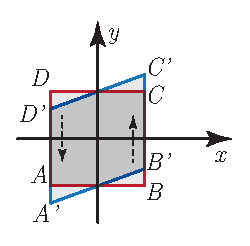
\includegraphics[scale=1]{figs/nyiras.eps}
\caption{Egytengelyű, egyszerű nyírás, az $y$ koordinátában az eltolás arányos $x$-szel}
\label{fig:nyiras}
\end{subfigure} \hfill
\begin{subfigure}[b]{0.45\textwidth}
\centering
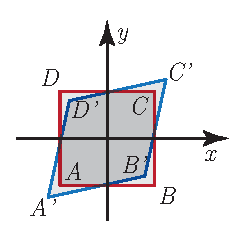
\includegraphics[scale=1]{figs/tiszta_nyiras.eps}
\caption{Tiszta nyírás, amely egy elforgatott, $45^\circ$-os koordináta-rendszerben nyújtás}
\label{fig:tiszta_nyiras}
\end{subfigure}
\label{fig_nyujtasok}
\caption{Nyírások szemléltetése.}
\end{figure}
\FloatBarrier

\footnotesize
\paragraph{Példa} Tekintsünk egy transzformációt, amit a ${\mathbf{F}} = \left( {\begin{array}{*{20}{c}}
  1&1 \\ 
  1&2 
\end{array}} \right)$ deformációs gradiens ad meg! Nyírás-e ez, és ha igen, milyen fajta? Rajzoljuk fel, hogy mibe viszi át az $ABCD$ négyzetet, aminek a sarkainak az $x$ és $y$ koordinátái a $\pm 1$-ben vannak!

\paragraph{Megoldás} Tiszta nyírás, mert a deformációs gradiens konstans és determinánsa 1. Az elmozdulásteret a
\[{{\mathbf{\beta }}^T} = {\mathbf{F}} - {\mathbf{I}} = \left( {\begin{array}{*{20}{c}}
  0&1 \\ 
  1&1 
\end{array}} \right)\]
disztorzióból kapjuk,
\[{\mathbf{u}}\left( {\mathbf{r}} \right) = \left( {\begin{array}{*{20}{c}}
  0&1 \\ 
  1&1 
\end{array}} \right)\left( {\begin{array}{*{20}{c}}
  x \\ 
  y 
\end{array}} \right) = \left( {\begin{array}{*{20}{c}}
  y \\ 
  {x + y} 
\end{array}} \right).\]
Így
\[\begin{gathered}
  \left( {\phantom{-}1,\phantom{-}1} \right) \mapsto \left( {2,3} \right) \hfill \\
  \left( { - 1,\phantom{-}1} \right) \mapsto \left( {0,1} \right) \hfill \\
  \left( { - 1, - 1} \right) \mapsto \left( { - 2, - 3} \right) \hfill \\
  \left( {\phantom{-}1, - 1} \right) \mapsto \left( {0, - 1} \right), \hfill \\ 
\end{gathered} \]
amelyet fel is rajzolhatunk:
\begin{figure}[htb] 
\centering
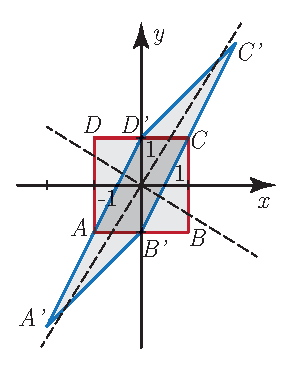
\includegraphics[scale=1]{figs/nyiras_feladat2.eps}
\caption{Tiszta nyírás, a nyújtás tengelyeinek a szöge nem nevezetes szög.}
\label{fig:nyiras_pelda2}
\end{figure}
\FloatBarrier
\normalsize

\subsubsection{Homokóra nyújtás}
Jobb kifejezés hiányában van ez a cím, lehetne még ferdítés. Ekkor a nyújtás mértéke lineárisan függ az egyik tengelytől, és arra merőleges. \Aref{fig:homokora_nyujtas_szamolos}.\ ábra egy ilyet szemléltet (a könnyebb ábrázolásért egy eltolással együtt), ahol a legkisebb $y$ értékű részét a térnek $0{,}75$ szorosára nyújtjuk, a legnagyobb $y$ értékű részt pedig $1{,}25$-szörösére nyújtottuk, a kettő között pedig lineáris az átmenet.
\begin{figure}[htb] 
\centering    
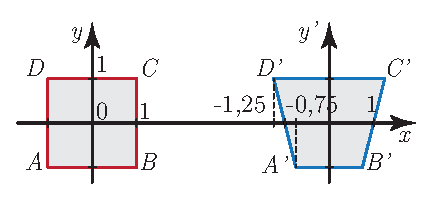
\includegraphics[scale=1]{figs/homokora_nyujtas_szamolos.eps}
\caption{A homokóra nyújtás példájának szemléltetése.}
\label{fig:homokora_nyujtas_szamolos}
\end{figure}

\footnotesize
\paragraph{Példa} az elmozdulástérre:
\[{\mathbf{u}}\left( {\mathbf{r}} \right) = \frac{1}{4}\left( {\begin{array}{*{20}{c}}
  {x \cdot y} \\ 
  0 
\end{array}} \right).\]
Ekkor a disztorziót deriválással lehet legkönnyebben megkapni,
\[\begin{gathered}
  {\partial _x}{u_x} = y/4 \hfill \\
  {\partial _y}{u_x} = x/4 \hfill \\
  {\partial _x}{u_y} = {\partial _y}{u_y} = 0, \hfill \\ 
\end{gathered} \]
így a disztorzióra és a deformációs gradiensre:
\[{{\mathbf{\beta }}^T} = \left( {\begin{array}{*{20}{c}}
  {y/4}&{x/4} \\ 
  0&0 
\end{array}} \right)\quad {\mathbf{F}} = \left( {\begin{array}{*{20}{c}}
  {1 + y/4}&{x/4} \\ 
  0&1 
\end{array}} \right).\]

Mi lenne, ha megint a $\Delta {\mathbf{r}}'$-ből szeretnénk számolni a disztorziót és a deformációs gradienst?
\[\Delta {\mathbf{r}}' = {{\mathbf{r}}_2}' - {{\mathbf{r}}_1}' = \left( {{{\mathbf{r}}_2} + {\mathbf{u}}\left( {{{\mathbf{r}}_2}} \right)} \right) - \left( {{{\mathbf{r}}_1} + {\mathbf{u}}\left( {{{\mathbf{r}}_1}} \right)} \right) = \Delta {\mathbf{r}} + {\mathbf{u}}\left( {{{\mathbf{r}}_2}} \right) - {\mathbf{u}}\left( {{{\mathbf{r}}_1}} \right)\]
Most nem tudunk továbblépni, mert ${\mathbf{u}}\left( {\mathbf{r}} \right)$ nem lineáris, azaz ${\mathbf{u}}\left( {\lambda {\mathbf{r}}} \right) \ne \lambda {\mathbf{u}}\left( {\mathbf{r}} \right)$. Továbbhaladni csak akkor tudunk, ha elvégezzük a $\Delta {\mathbf{r}}' \to 0$ limeszt, hogy lehessen aszerint osztani, pontosabban szólva deriválni:
\[d{\mathbf{r}}' = d{\mathbf{r}} + \frac{{{\mathbf{u}}\left( {{{\mathbf{r}}_2}} \right) - {\mathbf{u}}\left( {{{\mathbf{r}}_1}} \right)}}{{d{\mathbf{r}}}} = \left( {{\mathbf{I}} + \frac{{d{\mathbf{u}}\left( {\mathbf{r}} \right)}}{{d{\mathbf{r}}}}} \right)d{\mathbf{r}},\]
vagyis ezúttal is deriváláson keresztül tudunk csak számolni.

Nézzük meg, hogyan hat ez a transzformáció! Vegyünk egy négyzetet, amelynek a sarkainak a koordinátái legyenek 
\[{{\mathbf{r}}_A} = \left( {\begin{array}{*{20}{c}}
  { - 1} \\ 
  { - 1} 
\end{array}} \right)\quad {{\mathbf{r}}_B} = \left( {\begin{array}{*{20}{c}}
  1 \\ 
  { - 1} 
\end{array}} \right)\quad {{\mathbf{r}}_C} = \left( {\begin{array}{*{20}{c}}
  1 \\ 
  1 
\end{array}} \right)\quad {{\mathbf{r}}_D} = \left( {\begin{array}{*{20}{c}}
  { - 1} \\ 
  1 
\end{array}} \right).\]
Ekkor a transzformáció után a sarkok új koordinátáit az elmozdulástérből számolva:
\begin{alignat*}{2}
   & {\mathbf{u}}\left( {{{\mathbf{r}}_A}} \right) = {\mathbf{u}}\left( {\begin{array}{*{20}{c}}
  { - 1} \\ 
  { - 1} 
\end{array}} \right) = \frac{1}{4}\left( {\begin{array}{*{20}{c}}
  1 \\ 
  0 
\end{array}} \right)\quad  && {{\mathbf{r}}_A}' = \left( {\begin{array}{*{20}{c}}
  { - 1} \\ 
  { - 1} 
\end{array}} \right) + \frac{1}{4}\left( {\begin{array}{*{20}{c}}
  1 \\ 
  0 
\end{array}} \right) = \left( {\begin{array}{*{20}{c}}
  { - 0,75} \\ 
  { - 1} 
\end{array}} \right), \\ 
   & {\mathbf{u}}\left( {{{\mathbf{r}}_B}} \right) = {\mathbf{u}}\left( {\begin{array}{*{20}{c}}
  1 \\ 
  { - 1} 
\end{array}} \right) = \frac{1}{4}\left( {\begin{array}{*{20}{c}}
  { - 1} \\ 
  0 
\end{array}} \right)\quad  && {{\mathbf{r}}_B}' = \left( {\begin{array}{*{20}{c}}
  1 \\ 
  { - 1} 
\end{array}} \right) + \frac{1}{4}\left( {\begin{array}{*{20}{c}}
  { - 1} \\ 
  0 
\end{array}} \right) = \left( {\begin{array}{*{20}{c}}
  {0,75} \\ 
  { - 1} 
\end{array}} \right), \\ 
   & {\mathbf{u}}\left( {{{\mathbf{r}}_C}} \right) = {\mathbf{u}}\left( {\begin{array}{*{20}{c}}
  1 \\ 
  1 
\end{array}} \right) = \frac{1}{4}\left( {\begin{array}{*{20}{c}}
  1 \\ 
  0 
\end{array}} \right)\quad  && {{\mathbf{r}}_C}' = \left( {\begin{array}{*{20}{c}}
  1 \\ 
  1 
\end{array}} \right) + \frac{1}{4}\left( {\begin{array}{*{20}{c}}
  1 \\ 
  0 
\end{array}} \right) = \left( {\begin{array}{*{20}{c}}
  {1,25} \\ 
  { 1} 
\end{array}} \right), \\ 
   & {\mathbf{u}}\left( {{{\mathbf{r}}_D}} \right) = {\mathbf{u}}\left( {\begin{array}{*{20}{c}}
  { - 1} \\ 
  1 
\end{array}} \right) = \frac{1}{4}\left( {\begin{array}{*{20}{c}}
  { - 1} \\ 
  0 
\end{array}} \right)\quad  && {{\mathbf{r}}_D}' = \left( {\begin{array}{*{20}{c}}
  { - 1} \\ 
  1 
\end{array}} \right) + \frac{1}{4}\left( {\begin{array}{*{20}{c}}
  { - 1} \\ 
  0 
\end{array}} \right) = \left( {\begin{array}{*{20}{c}}
  { - 1,25} \\ 
  { 1} 
\end{array}} \right).
\end{alignat*}
Ezeket az értékeket nem kaphattuk volna meg abból, hogyha megadjuk az ${\mathbf{F}}$ vagy a ${\mathbf{\beta }}$ értékeit a négy sarokban, mert ezek az operátorok az adott helyben definiált $\Delta {\mathbf{r}}$ vektorra hatnak. A deformációs gradiens értékei az egyes sarkokban:
\[{{\mathbf{F}}_A} = \frac{1}{4}\left( {\begin{array}{*{20}{c}}
  3&{ - 1} \\ 
  0&4 
\end{array}} \right)\quad {{\mathbf{F}}_B} = \frac{1}{4}\left( {\begin{array}{*{20}{c}}
  3&1 \\ 
  0&4 
\end{array}} \right)\quad {{\mathbf{F}}_C} = \frac{1}{4}\left( {\begin{array}{*{20}{c}}
  5&1 \\ 
  0&4 
\end{array}} \right)\quad {{\mathbf{F}}_D} = \frac{1}{4}\left( {\begin{array}{*{20}{c}}
  5&{ - 1} \\ 
  0&4 
\end{array}} \right),\]
illetve
\[{\mathbf{\beta }}_A^T = \frac{1}{4}\left( {\begin{array}{*{20}{c}}
  { - 1}&{ - 1} \\ 
  0&0 
\end{array}} \right)\quad {\mathbf{\beta }}_B^T = \frac{1}{4}\left( {\begin{array}{*{20}{c}}
  { - 1}&1 \\ 
  0&0 
\end{array}} \right)\quad {\mathbf{\beta }}_C^T = \frac{1}{4}\left( {\begin{array}{*{20}{c}}
  1&1 \\ 
  0&0 
\end{array}} \right)\quad {\mathbf{\beta }}_D^T = \frac{1}{4}\left( {\begin{array}{*{20}{c}}
  1&{ - 1} \\ 
  0&0 
\end{array}} \right),\]
a négyzet közepén viszont \[{{\mathbf{F}}_0} = {\mathbf{I}}\quad {\mathbf{\beta_0 }} = 0,\]
így itt nincs deformáció. Ha veszek egy olyan $\Delta {\mathbf{r}}$ vektort, ami az origóból indul és a négyzet sarkára mutat, akkor a különböző részein különböző volna a deformáció.
\normalsize

\subsubsection{Csavarás}
A csavarás $3D$-ban értelmezhető transzformáció, amelynek során egy tengely mentén ugyanazon tengely irányában forgatunk, és a forgatás mértéke az anyag tengely menti két vége között folytonosan változik, legegyszerűbb esetben lineárisan.

Képzeljünk el egy $z$ tengelyű négyzetes hasábot, amely $z$-ben $-z_0$-tól $z_0$-ig terjed. Ekkor ennek minden $z$ síkbeli keresztmetszete négyzet. Forgassuk el a $-z_0$-ban lévő részét $z$ tengely mentén $-\alpha$ szöggel, azaz arra a síklapra alkalmazzunk egy ${{\mathbf{O}}_{z, - \alpha }}$ transzformációt. A $z_0$-ban lévő részét szintén $z$ tengely körül, de $\alpha$ szöggel. $-z_0$ és $z_0$ között pedig minden további keresztmetszetében lineárisan változzon a szög $-\alpha$ és $\alpha$ között, azaz pl.\ a $z^*$ keresztmetszeten egy 
\begin{equation}
\left( {\begin{array}{*{20}{c}}
  x \\ 
  y \\ 
  {{z^ * }} 
\end{array}} \right)' = {{\mathbf{O}}_{z,\alpha  \cdot {z^ * }/z_0}} \left( {\begin{array}{*{20}{c}}
  x \\ 
  y \\ 
  {{z^ * }} 
\end{array}} \right)
\end{equation}
forgatást hajtunk végre. Ez az egytengelyű csavarás.

Mi az elmozdulásmező, a deformációs gradiens, a disztorzió és a deformáció?

A koordináta rendszert úgy veszem fel, hogy a $z$ tengely a forgatás tengelye legyen, a minta tartománya pedig $-z_0$-tól $z_0$-ig tartson. Ekkor a ${\mathbf{r}} = \left( {\begin{array}{*{20}{c}}
  x&y&z 
\end{array}} \right)$ helyvektor $z$ koordinátája nem változik, csupán az $x$ és $y$ koordinátája, ${\mathbf{r}}' = \left( {\begin{array}{*{20}{c}}
  {x'}&{y'}&z 
\end{array}} \right)$. A vesszősök között a ${{\mathbf{O}}_{z,\alpha z/{z_0}}}$ hat, 
\[\left( {\begin{array}{*{20}{c}}
  {x'} \\ 
  {y'} 
\end{array}} \right) = \left( {\begin{array}{*{20}{c}}
  {\cos \left( {\alpha z/{z_0}} \right)}&{ - \sin \left( {\alpha z/{z_0}} \right)} \\ 
  {\sin \left( {\alpha z/{z_0}} \right)}&{\cos \left( {\alpha z/{z_0}} \right)} 
\end{array}} \right)\left( {\begin{array}{*{20}{c}}
  x \\ 
  y 
\end{array}} \right).\]
Ennek 3D-s kiterjesztése:
\[\left( {\begin{array}{*{20}{c}}
  {x'} \\ 
  {y'} \\ 
  z 
\end{array}} \right) = \underbrace {\left( {\begin{array}{*{20}{c}}
  {\cos \left( {\alpha z/{z_0}} \right)}&{ - \sin \left( {\alpha z/{z_0}} \right)}&0 \\ 
  {\sin \left( {\alpha z/{z_0}} \right)}&{\cos \left( {\alpha z/{z_0}} \right)}&0 \\ 
  0&0&1 
\end{array}} \right)}_{{\mathbf{O}}_{z,\alpha z/{z_0}}^{3D}}\left( {\begin{array}{*{20}{c}}
  x \\ 
  y \\ 
  z 
\end{array}} \right)\]
Az elmozdulástér tehát:
\[{\mathbf{r}}' = {\mathbf{O}}_{z,\alpha z/{z_0}}^{3D}\left( {\mathbf{r}} \right){\mathbf{r}} = {\mathbf{u}}\left( {\mathbf{r}} \right) + {\mathbf{r}} \Rightarrow {\mathbf{u}}\left( {\mathbf{r}} \right) = \left( {{\mathbf{O}}_{z,\alpha z/{z_0}}^{3D}\left( {\mathbf{r}} \right) - {{\mathbf{I}}^{3D}}} \right){\mathbf{r}},\]
a komponensei kiírva:
\[\begin{aligned}
  \left( {{\mathbf{O}}_{z,\alpha z/{z_0}}^{3D}\left( {\mathbf{r}} \right) - {{\mathbf{I}}^{3D}}} \right){\mathbf{r}} &  = \left( {\begin{array}{*{20}{c}}
  {\cos \left( {\frac{{z\alpha }}{{{z_0}}}} \right) - 1}&{ - \sin \left( {\frac{{z\alpha }}{{{z_0}}}} \right)}&0 \\ 
  {\sin \left( {\frac{{z\alpha }}{{{z_0}}}} \right)}&{\cos \left( {\frac{{z\alpha }}{{{z_0}}}} \right) - 1}&0 \\ 
  0&0&{1 - 1} 
\end{array}} \right)\left( {\begin{array}{*{20}{c}}
  x \\ 
  y \\ 
  z 
\end{array}} \right) \\ 
   &  = \left( {\begin{array}{*{20}{c}}
  {x\left[ {\cos \left( {\frac{{z\alpha }}{{{z_0}}}} \right) - 1} \right] - y\sin \left( {\frac{{z\alpha }}{{{z_0}}}} \right)} \\ 
  {y\left[ {\cos \left( {\frac{{z\alpha }}{{{z_0}}}} \right) - 1} \right] + x\sin \left( {\frac{{z\alpha }}{{{z_0}}}} \right)} \\ 
  0 
\end{array}} \right) = {\mathbf{u}}\left( {\mathbf{r}} \right) \\ 
\end{aligned} .\]
Irány derviálni! ${\beta^T _{ij}} = {\partial _j}{u_i}$
\begin{equation} \label{eq:csavaras_disztorzio}
\left( {\begin{array}{*{20}{c}}
  {\underbrace {\cos \left( {\frac{{z\alpha }}{{{z_0}}}} \right) - 1}_{{\partial _x}{u_x}}}&{\underbrace { - \sin \left( {\frac{{z\alpha }}{{{z_0}}}} \right)}_{{\partial _y}{u_x}}}&{\underbrace { - y\frac{\alpha }{{{z_0}}}\cos \left( {\frac{{z\alpha }}{{{z_0}}}} \right) - x\frac{\alpha }{{{z_0}}}\sin \left( {\frac{{z\alpha }}{{{z_0}}}} \right)}_{{\partial _z}{u_x}}} \\ 
  {\underbrace {\sin \left( {\frac{{z\alpha }}{{{z_0}}}} \right)}_{{\partial _x}{u_y}}}&{\underbrace {\cos \left( {\frac{{z\alpha }}{{{z_0}}}} \right) - 1}_{{\partial _y}{u_y}}}&{\underbrace {x\frac{\alpha }{{{z_0}}}\cos \left( {\frac{{z\alpha }}{{{z_0}}}} \right) - y\frac{\alpha }{{{z_0}}}\sin \left( {\frac{{z\alpha }}{{{z_0}}}} \right)}_{{\partial _z}{u_y}}} \\ 
  0&0&0 
\end{array}} \right) = {{\mathbf{\beta }}^T}
\end{equation}

Innen fáradtságos számolással megkapható a deformáció,
\[2{\mathbf{\varepsilon }} = {\mathbf{\beta }} + {{\mathbf{\beta }}^T} + {\mathbf{\beta }}{{\mathbf{\beta }}^T}.\]

\paragraph{Infinitezimális csavarás}
Infinitezimális csavarás esetén a szögelfordulás $\alpha$ értéke kicsi. Egyszerűsödik a disztrozió \aref{eq:csavaras_disztorzio}.\ kifejezése is, ha ${\mathbf{\beta }^T}$ kicsi, mert akkor egyrészt a disztrozió is egyszerűbb, határértékben

\[{{\mathbf{\beta }}^T} = \left( {\begin{array}{*{20}{c}}
  0&{ - \frac{{z\alpha }}{{{z_0}}}}&{ - y\frac{\alpha }{{{z_0}}} - x\frac{\alpha }{{{z_0}}}\frac{{z\alpha }}{{{z_0}}}} \\ 
  {\frac{{z\alpha }}{{{z_0}}}}&0&{x\frac{\alpha }{{{z_0}}} - y\frac{\alpha }{{{z_0}}}\frac{{z\alpha }}{{{z_0}}}} \\ 
  0&0&0 
\end{array}} \right) = \left( {\begin{array}{*{20}{c}}
  0&{ - \frac{{z\alpha }}{{{z_0}}}}&{ - y\frac{\alpha }{{{z_0}}}} \\ 
  {\frac{{z\alpha }}{{{z_0}}}}&0&{x\frac{\alpha }{{{z_0}}}} \\ 
  0&0&0 
\end{array}} \right),\]
másrészt a deformációban nincs meg a csúnya ${\mathbf{\beta }}{{\mathbf{\beta }}^T}$ szorzat, 
\[2{\mathbf{\varepsilon }} = {\mathbf{\beta }} + {{\mathbf{\beta }}^T}.\]
Kiszámolva:
\[{\mathbf{\varepsilon }} = \left( {\begin{array}{*{20}{c}}
  0&0&{ - y\frac{\alpha }{{2{z_0}}}} \\ 
  0&0&{x\frac{\alpha }{{2{z_0}}}} \\ 
  { - y\frac{\alpha }{{2{z_0}}}}&{x\frac{\alpha }{{2{z_0}}}}&0 
\end{array}} \right).\]
Ekkor egyébként az elmozdulástér határértékben:
\[{\mathbf{u}}\left( {\mathbf{r}} \right) = \left( {\begin{array}{*{20}{c}}
  { - yz \cdot \alpha /{z_0}} \\ 
  {xz \cdot \alpha /{z_0}} \\ 
  0 
\end{array}} \right).\]
Persze egyszerűbb lett volna ezt deriválni.

\subsubsection{Lineárisan interpolált transzformációk}
Még megannyi más deformáció fajta is elképzelhető. Volna lehetőség arra, hogy megadjuk például, hogy a transzformáció mibe viszi át az egységnégyzetet. Ez jóval szemléletesebb, mint az ${\mathbf{F}}\left( {\mathbf{r}} \right)$ vagy az ${\mathbf{\varepsilon }}\left( {\mathbf{r}} \right)$ függvény megadása, viszont nem következik belőle a transzformáció pontos alakja. Amennyiben a transzformációt mégis ilyen vizuális úton adjuk meg, akkor arra egyszerű esetekben egy lehetőség, hogy megadjuk, hogy az egyes oldalakat mennyire nyújtotta meg a transzformáció, majd minden pontra lineáris interpolációval meghatározhatnánk az abban a pontban érvényes elmozdulás értékét.

\begin{figure}[htb] 
\centering    
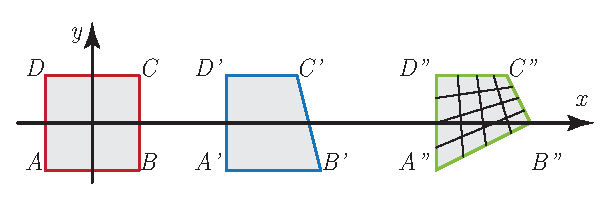
\includegraphics[scale=1]{figs/linearisan_interpolalt.eps}
\caption{Az elmozdulásmezőt lineárisan interpolálhatjuk az oldalélek között.}
\label{fig:linearis_interpolacios_traf}
\end{figure}

\subsubsection{Általános transzformációk}
Mint ahogy egy függvény közelíthetünk szakaszonként egy konstans értékkel, egy transzformációt is közelíthetünk helyről helyre konstans térben konstans transzformációval, mondjuk az ${\mathbf{F}}$ deformációs gradiens megadásával, így helyről helyre különböző mértékű, többtengelyű nyújtással és forgatással írhatjuk le a transzformációt.

Érezhető, hogy amennyiben egy függvényt konstans értékek halmazával akarunk leírni, akkor sok pont kell. Kevesebb adattal leírható egy függvény, ha egyeneseket használunk a leírására, és abból állítjuk elő a függvényt (a megfelelő szempontból, ha a függvény elég jól viselkedik). Hasonlóképp egy fokkal magasabb szinten írjuk le a transzformációt, ha nem konstans értékű transzformációkkal közelítjük, hanem lineárissal. Ekkor a homokóra nyújtás kéttengelyű esetét használják. 

\subsection{Transzformációk egymásutánja}
Ha alkalmazunk egy transzformációt a mintán, majd az így kapotton újra, akkor az egyes transzformációhoz tartozó deformációs gradienst (ill.\ a transzponáltjaikat) össze kell szorozni \az{\eqref{eq:disztrozio_def}} egyenlet szerint, hogy megkapjuk $\Delta {\mathbf{r}}''$-t:
\[1 + {{\mathbf{\beta }}_{AB}} = \left( {1 + {{\mathbf{\beta }}_B}} \right)\left( {1 + {{\mathbf{\beta }}_A}} \right) = \left( {1 + {{\mathbf{\beta }}_A} + {{\mathbf{\beta }}_B} + {{\mathbf{\beta }}_B}{{\mathbf{\beta }}_A}} \right) \ne 1 + {{\mathbf{\beta }}_{BA}}.\]
Láthatjuk, hogy ez nem kommutatív, a transzformációk egymással nem felcserélhetők. Azonban ha a disztorzió elég kicsi, és így a szorzatuk elhanyagolható, akkor már kommutatív, ugyanis 
\begin{equation} \label{eq:deform_kommutatív}
1 + {{\mathbf{\beta }}_{AB}} = \left( {1 + {{\mathbf{\beta }}_A}} \right)\left( {1 + {{\mathbf{\beta }}_B}} \right) = \left( {1 + {{\mathbf{\beta }}_A} + {{\mathbf{\beta }}_B}\underbrace { + {{\mathbf{\beta }}_A}{{\mathbf{\beta }}_B}}_{ \approx 0}} \right) = 1 + {{\mathbf{\beta }}_A} + {{\mathbf{\beta }}_B} = 1 + {{\mathbf{\beta }}_{BA}}.
\end{equation}
(Mit jelent ez a deformációs gradiensre és a deformációra nézve?)

Egy forgatás nem hoz létre deformációt. Ha a transzformáció nem tisztán forgatást ír le, akkor a tisztán forgatást leíró része nem hoz létre deformációt, csak a maradék. Mi az, hogy része? Hogyan hattathatóak a transzformációk egymás után, és hogyan olvasható le, hogy mekkora az eredő deformáció?

\subsubsection{Poláris dekompozíció} \label{sec:polaris_dekomp}
\Az{\eqref{eq:disztrozio_def}} egyenletből láthatóan az ${\mathbf{F}} = 1 + {{\mathbf{\beta }}^T}$ mennyiségek összeszorzódnak. Jelöljön ${\mathbf{O}}$ egy ortogonális mátrixot (ilyenek voltak a forgatásnak a transzformációs mátrixai), ${\mathbf{U}}$ pedig egy szimmetrikus mátrixot (ilyenek voltak a tiszta nyújtás mátrixai)! Megmutatjuk, hogyha ${\mathbf{F}}$ invertálható, akkor (egyértelműen) felírható ${\mathbf{F}} = {\mathbf{OU}}$ alakban!
Legyen
\begin{equation} \label{eq:szimm_def_grad}
{{\mathbf{F}}^T}{\mathbf{F}} = {\mathbf{VD}}{{\mathbf{V}}^T},
\end{equation}
ahol ${\mathbf{V}}$ ortogonális, ${{\mathbf{D}}}$ pedig diagonális mátrix\footnote{Egy diagonális mátrixon értelmezett függvény az egyes mátrixkomponensek ugyanazon függvénye.} Ezt megtehetjük, hisz ${{\mathbf{F}}^T}{\mathbf{F}}$ szimmetrikus, mi több, pozitív definit, így nem csak diagonalizálható, de abból gyököt is vonhatunk, és az inverzét is vehetjük. Így van értelme és igaz az alábbi azonosság:
\[{\mathbf{F}} = \underbrace {{\mathbf{F}}{{\left( {{{\mathbf{F}}^T}{\mathbf{F}}} \right)}^{ - 1/2}}}_{\mathbf{O}}\underbrace {{{\left( {{{\mathbf{F}}^T}{\mathbf{F}}} \right)}^{1/2}}}_{\mathbf{U}},\]
ahol bevezettünk két mátrixot, ${\mathbf{O}}$-t és ${\mathbf{U}}$-t. Most pedig belátjuk, hogy ${\mathbf{U}}$ szimmetrikus, illetve, hogy ${\mathbf{O}}$ ortogonális.

Az ${\mathbf{U}}$ szimmetrikusságának megmutatásához először el kell végeznünk \az{\eqref{eq:szimm_def_grad}}.\ egyenlet mindkét oldalán egy gyökvonást, mert
\begin{equation} \label{eq:Udef}
{\mathbf{U}} = {\left( {{{\mathbf{F}}^T}{\mathbf{F}}} \right)^{1/2}} = {\left( {{\mathbf{VD}}{{\mathbf{V}}^T}} \right)^{1/2}}.
\end{equation}
Ezt úgy tehetjük meg, hogyha a gyököt csak a diagonális mátrixra hattatjuk, azaz
\begin{equation} \label{eq:diag_m_fgv}
{\left( {{\mathbf{VD}}{{\mathbf{V}}^T}} \right)^{1/2}} = {\mathbf{V}}{{\mathbf{D}}^{1/2}}{{\mathbf{V}}^T}.
\end{equation}
Ellenőrzésképp nézzük meg, hogy mit ad ennek a mátrixnak az önmagával vett szorzata!
\[
  {\mathbf{V}}\overbrace {{{\mathbf{D}}^{1/2}}\underbrace {{{\mathbf{V}}^T} \cdot {\mathbf{V}}}_{\mathbf{I}}{{\mathbf{D}}^{1/2}}}^{\mathbf{D}}{{\mathbf{V}}^T} = {\mathbf{VD}}{{\mathbf{V}}^T} = {{\mathbf{F}}^T}{\mathbf{F}}.
\]
Tehát ez valóban a négyzetgyöke, mert a négyzete épp ${{{\mathbf{F}}^T}{\mathbf{F}}}$. Most számítsuk ki ${{\mathbf{U}}^T}$-t \told{\aref({eq:Udef})}+as{} definíció és \told{\aref({eq:diag_m_fgv})}+as{} eredmény felhasználásával!
\[{{\mathbf{U}}^T} = {\left( {{\mathbf{V}}{{\mathbf{D}}^{1/2}}{{\mathbf{V}}^T}} \right)^T} = {\left( {{{\mathbf{V}}^T}} \right)^T}{\left( {{{\mathbf{D}}^{1/2}}} \right)^T}{{\mathbf{V}}^T} = {\mathbf{V}}{{\mathbf{D}}^{1/2}}{{\mathbf{V}}^T} = {{\mathbf{U}}},\]
azaz ${\mathbf{U}} = {{\mathbf{U}}^T}$, tehát ${\mathbf{U}}$ szimmetrikus.

Most belátjuk, hogy ${\mathbf{O}}$ ortogonális! \Az{\eqref{eq:diag_m_fgv}}.\ egyenlethez hasonlóan, az inverz gyökét \az{\eqref{eq:szimm_def_grad}}.\ egyenletnek úgy vehetjük, hogyha a diagonális mátrixnak vesszük az inverzének a gyökét, vagyis
\[{\left( {{{\mathbf{F}}^T}{\mathbf{F}}} \right)^{ - 1/2}} = {\mathbf{V}}{{\mathbf{D}}^{ - 1/2}}{{\mathbf{V}}^T}.\]
Ellenőrzésképp nézzük meg, hogy mit ad ennek a mátrixnak a szorzata az inverzével, vagyis!
\[{\left( {{{\mathbf{F}}^T}{\mathbf{F}}} \right)^{ - 1/2}}{\left( {{{\mathbf{F}}^T}{\mathbf{F}}} \right)^{1/2}} = {\mathbf{V}}\overbrace {{{\mathbf{D}}^{ - 1/2}}\underbrace {{{\mathbf{V}}^T} \cdot {\mathbf{V}}}_{\mathbf{I}}{{\mathbf{D}}^{1/2}}}^{\mathbf{I}}{{\mathbf{V}}^T} = {\mathbf{V}}{{\mathbf{V}}^T} = {\mathbf{I}}.\]
Tehát valóban jól írtuk fel az inverz gyökét. Már csak be kell látni, hogy ${\mathbf{O}}$ ortogonális. Ehhez ${\mathbf{O}}$-t balról megszorozva a transzponáltjával kapjuk, hogy
\begin{multline*}
{\left( {{\mathbf{F}}{{\left( {{{\mathbf{F}}^T}{\mathbf{F}}} \right)}^{ - 1/2}}} \right)^T} \cdot {\mathbf{F}}{\left( {{{\mathbf{F}}^T}{\mathbf{F}}} \right)^{ - 1/2}} = {\left( {{\mathbf{V}}{{\mathbf{D}}^{ - 1/2}}{{\mathbf{V}}^T}} \right)^T}\underbrace {{{\mathbf{F}}^T} \cdot {\mathbf{F}}}_{{\mathbf{VD}}{{\mathbf{V}}^T}}{\mathbf{V}}{{\mathbf{D}}^{ - 1/2}}{{\mathbf{V}}^T} = \\ = {\mathbf{V}}\overbrace {{{\mathbf{D}}^{ - 1/2}}\underbrace {{{\mathbf{V}}^T}{\mathbf{V}}}_{\mathbf{I}}{\mathbf{D}}\underbrace {{{\mathbf{V}}^T}{\mathbf{V}}}_{\mathbf{I}}{{\mathbf{D}}^{ - 1/2}}}^{\mathbf{I}}{{\mathbf{V}}^T} = {\mathbf{V}}{{\mathbf{V}}^T} = {\mathbf{I}},
\end{multline*}
vagyis ${{\mathbf{O}}^T}{\mathbf{O}} = {\mathbf{I}}$, azaz ${\mathbf{O}}$ ortogonális.

Hogyan kaphatjuk tehát meg egy általános ${\mathbf{F}}$-ből, hogy milyen nyújtást és forgatást ír le? A lépések:
\begin{enumerate}
\item ${{{\mathbf{F}}^T}{\mathbf{F}}}$ kiszámolása.
\item Az így kapott szimmetrikus mátrix diagonalizálása egy ${\mathbf{V}}$ és ${\mathbf{V^T}}$ mátrixokkal, ekkor megkapjuk ${\mathbf{D}}$-t.
\item A diagonális mátrix gyökének és az inverzének a gyökének a kiszámítása ${{\mathbf{D}}^{1/2}}$ és ${{\mathbf{D}}^{ - 1/2}}$-hez. Ezt megtehetjük elemenként.
\item Visszaforgatjuk ezeket a mátrixokat az eredeti vonatkoztatási rendszerbe, ebből ${\mathbf{U}}$-t egyből, ${\mathbf{O}}$-t pedig egy balról vett ${\mathbf{F}}$-fel való szorzással kapjuk meg,
\[\begin{aligned}
  {\mathbf{U}} &  = {\mathbf{V}}{{\mathbf{D}}^{1/2}}{{\mathbf{V}}^T} \\ 
  {\mathbf{O}} &  = {\mathbf{F}} \cdot {\mathbf{V}}{{\mathbf{D}}^{ - 1/2}}{{\mathbf{V}}^T}. \\ 
\end{aligned} \]
\end{enumerate}

\footnotesize
\paragraph{Példa} Tekintsünk egy transzformációt, amit a ${\mathbf{F}} = \left( {\begin{array}{*{20}{c}}
  1&1 \\ 
  1&2 
\end{array}} \right)$ deformációs gradiens ad meg! Milyen fajta transzformáció ez? Rajzoljuk fel, hogy mibe viszi át az $ABCD$ négyzetet, aminek a sarkainak az $x$ és $y$ koordinátái a $\pm 1$-ben vannak! Tartalmaz-e forgatást vagy nyújtást a transzformáció, és ha igen, adjuk meg ezeket! Mekkora a nyújtás tengelyeinek $x$ tengellyel bezárt szöge?

\paragraph{Megoldás} A deformációs gradiens szimmetrikus és 1 determinánsú, így tiszta nyírás, avagy nyújtás, forgatást nem tartalmaz, avagy a forgatáshoz tartozó operátor az identitás operátor. A deformációs gradiens sajátértékei a $\lambda_a = \left( {3 + \sqrt 5 } \right)/2$ és a $\lambda_b = \left( {3 - \sqrt 5 } \right)/2$, a hozzájuk tartozó sajátvektorok pedig
\[{{\mathbf{v}}_a} = \frac{1}{{\sqrt {4 + {{\left( {\sqrt 5  - 1} \right)}^2}} }} \cdot \left( {\begin{array}{*{20}{c}}
  {\sqrt 5  - 1} \\ 
  2 
\end{array}} \right)\quad \quad {{\mathbf{v}}_b} = \frac{1}{{\sqrt {4 + {{\left( {\sqrt 5  + 1} \right)}^2}} }} \cdot \left( {\begin{array}{*{20}{c}}
  {\sqrt 5  + 1} \\ 
  { - 2} 
\end{array}} \right).\]
Ezek $x$ tengellyel bezárt szögei $\arctan \left( {2/\left( {\sqrt 5  - 1} \right)} \right) \approx 58^\circ $, illetve az ezzel  $90^\circ$-ot bezáró, $-32^\circ$-ot bezáró tengelyek. A megoldás szemléltetéséhez tekintsük \aref{fig:nyiras_pelda2}.\ ábrát! Ha a transzformáció tartalmazott volna forgatást is, akkor nem lett volna ${\mathbf{F}}$ szimmetrikus, és így nem lett volna diagonalizálható sem, így nem ${\mathbf{F}}$-nek, hanem ${{\mathbf{F}}^T}{\mathbf{F}}$ szorzatnak kellett volna megkeresni a sajátértékeit és sajátvektorait.
\paragraph{Példa} Tekintsünk egy egytengelyű nyírást, amelyet a ${\mathbf{F}} = \left( {\begin{array}{*{20}{c}}
  1&a  \\ 
  0&1 
\end{array}} \right)$ deformációs gradiens jellemez, amelyben $a$ egy másodrendben kicsi paraméter. Fejezzük ki, hogy mekkora nyújtást és forgatást tartalmaz ez a transzformáció annak segítségével, hogy felírjuk a nyújtást leíró mátrixot abban a vonatkoztatási rendszerben, amelyben az diagonális, majd adjuk meg a forgatást leíró részét, elsőrendig közelítve. \textbf{Tipp:} minden lépésben elhanyagolhatjuk az $a$-ban magasabbrendű tagokat.
\paragraph{Megoldás} Felírva ${{\mathbf{F}}^T}{\mathbf{F}}$-et, annak sajátvektorai (elsőrendig közelítve) a
\[{{\mathbf{v}}_\alpha } = \frac{1}{{\sqrt 2 }}\left( {\begin{array}{*{20}{c}}
  { - 1 - a/4} \\ 
  {1 - a/4} 
\end{array}} \right)\quad \quad {{\mathbf{v}}_\beta } = \frac{1}{{\sqrt 2 }}\left( {\begin{array}{*{20}{c}}
  {1 - a/4} \\ 
  {1 + a/4} 
\end{array}} \right)\]
vektorok. Azonban ha már ${{\mathbf{F}}^T}{\mathbf{F}}$-et linearizáljuk, akkor a sajátvektorok elsőrendben $a$-tól függetlenek lesznek ($a=0$ helyettesítést kell beírni az előbbi összefüggésbe). Így a transzformáció ${{\mathbf{F}}^T}{\mathbf{F}}$ diagonális alakjára kapjuk, hogy
\[{\mathbf{D}} = \frac{1}{2}\left( {\begin{array}{*{20}{c}}
  {2 + a\left( {a - \sqrt {4 + {a^2}} } \right)}&0 \\ 
  0&{2 + a\left( {a + \sqrt {4 + {a^2}} } \right)} 
\end{array}} \right) \approx \left( {\begin{array}{*{20}{c}}
  {1 - a}&0 \\ 
  0&{1 + a} 
\end{array}} \right).\]
Ennek a gyökét tagonként vehetjük, majd $a \approx 0$ körül 1.\ rendben sorfejtve, azaz a lineáris tagokat megtartva kapjuk, hogy
\[{{\mathbf{D}}^{1/2}} \approx \left( {\begin{array}{*{20}{c}}
  {1 - a/2}&0 \\ 
  0&{1 + a/2} 
\end{array}} \right).\]
A forgatás operátor tagjait kifejezve első rendig pedig azt kapjuk, hogy 
\[{\mathbf{O}} = \left( {\begin{array}{*{20}{c}}
  1&{a/2} \\ 
  { - a/2}&1 
\end{array}} \right).\]
\normalsize

\subsubsection{A nemkommutativitás szemléltetése}
Felmerülhet a kérdés, hogy miért épp ${\mathbf{F}} = {\mathbf{OU}}$ alakban bontottuk fel egy általános trasznformációt és miért nem ${\mathbf{F}} = {\mathbf{UO}}$ alakban. Egyáltalán lehetséges egy ilyen felbontás is? És ha igen, mi a különbség?

Még általánosabban felmerülhet a kérdés, hogy mi a szerepe a transzformációk sorrendjének. Nem mindegy, hogy először nyújtom, aztán forgatom, vagy először forgatom, aztán nyújtom?

\footnotesize
\paragraph{Példa}
Tekintsük az $x$ irányban kétszeresre nyújtó ${{\mathbf{U}}_2}$, és $z$ tengely kürül $30^\circ$-kal forgató ${{\mathbf{O}}_{z,30^\circ }}$ transzformációt leíró deformációs gradienseket! Ha először nyújtok, aztán forgatok, akkor az eredő deformációs gradiens
\[\begin{aligned}
  {{\mathbf{F}}_{2{\text{ majd }}z,30^\circ }} &  = {{\mathbf{O}}_{z,30^\circ }}{{\mathbf{U}}_2} =  {{\mathbf{F}}_{{\mathbf{OU}}}} = \left( {\begin{array}{*{20}{c}}
  {\cos \left( {30^\circ } \right)}&{ - \sin \left( {30^\circ } \right)} \\ 
  {\sin \left( {30^\circ } \right)}&{\cos \left( {30^\circ } \right)} 
\end{array}} \right)\left( {\begin{array}{*{20}{c}}
  2&0 \\ 
  0&1 
\end{array}} \right) \\ 
   &  = \left( {\begin{array}{*{20}{c}}
  {2\cos \left( {30^\circ } \right)}&{ - \sin \left( {30^\circ } \right)} \\ 
  {2\sin \left( {30^\circ } \right)}&{\cos \left( {30^\circ } \right)} 
\end{array}} \right). \\ 
\end{aligned} \]

Ezzel szenmben, ha először forgatok, aztán nyújtok:
\[\begin{aligned}
  {{\mathbf{F}}_{z,30^\circ {\text{ majd 2}}}} &  = {{\mathbf{U}}_2}{{\mathbf{O}}_{z,30^\circ }} = {{\mathbf{F}}_{{\mathbf{UO}}}} = \left( {\begin{array}{*{20}{c}}
  2&0 \\ 
  0&1 
\end{array}} \right)\left( {\begin{array}{*{20}{c}}
  {\cos \left( {30^\circ } \right)}&{ - \sin \left( {30^\circ } \right)} \\ 
  {\sin \left( {30^\circ } \right)}&{\cos \left( {30^\circ } \right)} 
\end{array}} \right) \\ 
   &  = \left( {\begin{array}{*{20}{c}}
  {2\cos \left( {30^\circ } \right)}&{ - 2\sin \left( {30^\circ } \right)} \\ 
  {\sin \left( {30^\circ } \right)}&{\cos \left( {30^\circ } \right)} 
\end{array}} \right). \\ 
\end{aligned} \]
Láthatjuk, hogy a két deformációs gradiens nem egyezik meg. Nézzük meg, hogy mibe viszi át az egyik, illetve másik transzformáció az  origóra tett négyzetet (legalábbis a jobb felső sarkát)! Ehhez először találjuk ki az elmozdulásmezőt az ${\mathbf{F}} = {\mathbf{I}} + \frac{{d{\mathbf{u}}}}{{d{\mathbf{r}}}}$ összefüggésből:
 \[\begin{gathered}
  {{\mathbf{u}}_{{\mathbf{OU}}}} = \left( {\begin{array}{*{20}{c}}
  {2\cos \left( {30^\circ } \right) - 1}&{ - \sin \left( {30^\circ } \right)} \\ 
  {2\sin \left( {30^\circ } \right)}&{\cos \left( {30^\circ } \right) - 1} 
\end{array}} \right)\left( {\begin{array}{*{20}{c}}
  x \\ 
  y 
\end{array}} \right), \hfill \\
  {{\mathbf{u}}_{{\mathbf{UO}}}} = \left( {\begin{array}{*{20}{c}}
  {2\cos \left( {30^\circ } \right) - 1}&{ - 2\sin \left( {30^\circ } \right)} \\ 
  {\sin \left( {30^\circ } \right)}&{\cos \left( {30^\circ } \right) - 1} 
\end{array}} \right)\left( {\begin{array}{*{20}{c}}
  x \\ 
  y 
\end{array}} \right). \hfill \\ 
\end{gathered} \]
A négyzet új sarka:
\[\begin{aligned}
  \left( {\begin{array}{*{20}{c}}
  1 \\ 
  1 
\end{array}} \right)' &  = \left( {\begin{array}{*{20}{c}}
  1 \\ 
  1 
\end{array}} \right) + {{\mathbf{u}}_{{\mathbf{OU}}}}\left( {\begin{array}{*{20}{c}}
  1 \\ 
  1 
\end{array}} \right) \\ 
   &  = \left( {{{\mathbf{u}}_{{\mathbf{OU}}}} + {\mathbf{I}}} \right)\left( {\begin{array}{*{20}{c}}
  1 \\ 
  1 
\end{array}} \right) \\ 
   &  = \left( {\begin{array}{*{20}{c}}
  {2\cos \left( {30^\circ } \right)}&{ - \sin \left( {30^\circ } \right)} \\ 
  {2\sin \left( {30^\circ } \right)}&{\cos \left( {30^\circ } \right)} 
\end{array}} \right)\left( {\begin{array}{*{20}{c}}
  1 \\ 
  1 
\end{array}} \right) = \left( {\begin{array}{*{20}{c}}
  {2\cos \left( {30^\circ } \right) - \sin \left( {30^\circ } \right)} \\ 
  {2\sin \left( {30^\circ } \right) + \cos \left( {30^\circ } \right)} 
\end{array}} \right). \\ 
\end{aligned} \]
Talán nem meglepő, hogy
\[\underbrace {\left( {\begin{array}{*{20}{c}}
  {\cos \left( {30^\circ } \right)}&{ - \sin \left( {30^\circ } \right)} \\ 
  {\sin \left( {30^\circ } \right)}&{\cos \left( {30^\circ } \right)} 
\end{array}} \right)}_{{{\mathbf{O}}_{z,30^\circ }}}\left( {\begin{array}{*{20}{c}}
  2 \\ 
  1 
\end{array}} \right) = \left( {\begin{array}{*{20}{c}}
  {2\cos \left( {30^\circ } \right) - \sin \left( {30^\circ } \right)} \\ 
  {2\sin \left( {30^\circ } \right) + \cos \left( {30^\circ } \right)} 
\end{array}} \right) = \left( {\begin{array}{*{20}{c}}
  1 \\ 
  1 
\end{array}} \right)',\]
vagyis azt kaptuk, az eredő transzformáció olyan, mintha a már megnyújtott teret elforgattuk volna.

Ha a transzformációkatt felcserélem, akkor
\[\begin{aligned}
  \left( {\begin{array}{*{20}{c}}
  1 \\ 
  1 
\end{array}} \right)' &  = \left( {\begin{array}{*{20}{c}}
  1 \\ 
  1 
\end{array}} \right) + {{\mathbf{u}}_{{\mathbf{UO}}}}\left( {\begin{array}{*{20}{c}}
  1 \\ 
  1 
\end{array}} \right) \\ 
   &  = \left( {{{\mathbf{u}}_{{\mathbf{UO}}}} + {\mathbf{I}}} \right)\left( {\begin{array}{*{20}{c}}
  1 \\ 
  1 
\end{array}} \right) \\ 
   &  = \left( {\begin{array}{*{20}{c}}
  {2\cos \left( {30^\circ } \right)}&{ - 2\sin \left( {30^\circ } \right)} \\ 
  {\sin \left( {30^\circ } \right)}&{\cos \left( {30^\circ } \right)} 
\end{array}} \right)\left( {\begin{array}{*{20}{c}}
  1 \\ 
  1 
\end{array}} \right) = \left( {\begin{array}{*{20}{c}}
  {2\cos \left( {30^\circ } \right) - 2\sin \left( {30^\circ } \right)} \\ 
  {\sin \left( {30^\circ } \right) + \cos \left( {30^\circ } \right)} 
\end{array}} \right), \\ 
\end{aligned} \]
amelyre pedig az igaz, hogy 
\[\left( {\begin{array}{*{20}{c}}
  2&0 \\ 
  0&1 
\end{array}} \right)\left( {\begin{array}{*{20}{c}}
  {\cos \left( {30^\circ } \right) - \sin \left( {30^\circ } \right)} \\ 
  {\sin \left( {30^\circ } \right) + \cos \left( {30^\circ } \right)} 
\end{array}} \right) = \left( {\begin{array}{*{20}{c}}
  {2\cos \left( {30^\circ } \right) - 2\sin \left( {30^\circ } \right)} \\ 
  {\sin \left( {30^\circ } \right) + \cos \left( {30^\circ } \right)} 
\end{array}} \right) = \left( {\begin{array}{*{20}{c}}
  1 \\ 
  1 
\end{array}} \right)',\]
vagyis azt kaptuk, hogy egy eleve elforgatott teret nyújtottunk meg. A nyújtás iránya azonban nem a négyzet oldalainak irányába mutat. Ez egészen pontosan azt jelenti, hogy abban a vonatkoztatási rendszerben, amelyben a négyzet oldalainak az iránya határozzák meg a vonatkoztatási rendszert, a nyújtási mátrix nem diagonális. A kétfajta transzformációt szemlélteti \aref{fig:nem_kommutativ}.\ ábra.
\normalsize

\begin{figure}[htb] 
\centering    
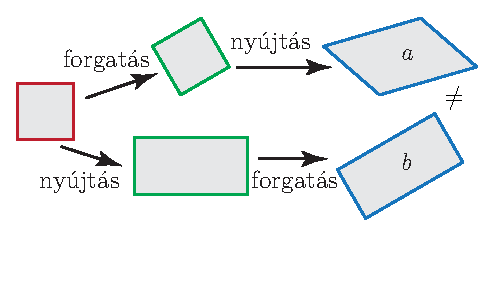
\includegraphics[scale=1]{figs/nem_kommutativ.eps}
\caption[Nem kommutatív transzformációk]{A transzformációk nem felcserélhetőségének illusztációja. A forgatást és nyújtást megadó mátrixok az eredeti vonatkoztatási rendszerben vannak megadva, azonban a testet a 2.\ transzformáció előtt már transzformáltuk egyszer, ellenben a koordinátarendszer nem változott.}
\label{fig:nem_kommutativ}
\end{figure}

Talán azért szokták először a nyújtás, majd a forgatást elvégezni, mert így az alakzat emberek számára könnyebben felismerhető, illetve vizuálisan az egyes transzformációk könnyebben leolvashatóak. \Aref{fig:nem_kommutativ}.\ ábra \textit{b} esetét előállíthatnánk egy forgatás és egy tiszta nyírás (amihez szintén egy ortogonális deformációs gradiens tartozik) egymásutánjaként, de ekkor a nyírás elemei nehezebben leolvashatók, az csak a $30^\circ$-os koordinátarendszerben diagonális.

\footnotesize
\paragraph{Példa}
\begin{enumerate}
\item Milyen transzformációk ismerhetőek fel \aref{fig:egymasutan}.\ ábráról?
\item Mi az elmozdulásmező, a deformációs gradiens, a disztorzió és a deformáció?
\end{enumerate}
\begin{figure}[htb] 
\centering    
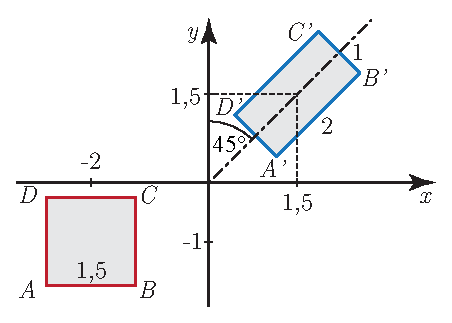
\includegraphics[scale=1]{figs/egymasutan_feladat.eps}
\caption{Egymásután.}
\label{fig:egymasutan}
\end{figure}
\FloatBarrier

\paragraph{Megoldás}
\begin{enumerate}
\item Az $x$ tengely mentén $4/3$-ad, $y$ tengely mentén $2/3$ szorosra nyújtás, $45^\circ $-kal való forgatás, majd eltolás $\left( {3{,}5;\;2{,}5} \right)$ vektorral.
\item Felírjuk a nyújtás majd forgatás deformációs gradienseinek a szorzatát. Ebből számolható az elmozdulásmező lineáris része, a konstans részét pedig úgy választjuk meg, hogy pl.\ az alakzat közepét jó helyre tegye.
\end{enumerate}
\normalsize


\section{Folytonos közegek egyensúlya}
Newton-tétele szerint egy pontszerű test gyorsulását a rá ható erők összessége adja meg. A tétel nagysága abban rejlik, hogy megadja, hogy az erők mitől függhetnek, több test esetén hogyan kezelendők, illetve hogyan összegezendők. A
\begin{equation} \label{eq:newton}
{\mathbf{F}} = m{\mathbf{a}}
\end{equation}
összefüggést írjuk kicsiny részek összegére, amelyben a tömeget valamilyen tömegsűrűség integrálja adja, illetve csoportosítsuk az erőket aszerint, hogy a pontszerű testre azon
\begin{itemize}
\item térfogatában hat, azaz nem a felülettel való érintkezés folyamán, hanem távolba hatás által (mint pl.\ gravitációs erő, elektrosztatikus erő), vagy
\item felületén keresztül hat, valamilyen kontakterő folyamán (Van der Waals erő, súrlódás, atomok közti vonzó vagy taszító erő, bár ezek mind ugyanolyan mikroszkopikus eredettel rendelkeznek).
\end{itemize}
Így egy, akár nagyobb testben lévő, általunk kijelölt kisebb testre ható eredő erő e kettő fajta erőnek az összege, az egyiket a felületre, a másikat a térfogatra kell összegezni,
\begin{equation} \label{eq:erok_csop}
{\mathbf{F}} = \underbrace {\int_{\partial V} {d{{\mathbf{F}}_f}} }_{{\text{felületi}}} + \underbrace {\int_V {d{{\mathbf{F}}_t}} }_{\text{térfogati}},
\end{equation}
amelyek közül a felületi erő arányos a kicsi felületi elemmel,
\[d{{\mathbf{F}}_f} \sim d{\mathbf{A}} \Leftrightarrow d{{\mathbf{F}}_f} = \hat \sigma \left( {\mathbf{r}} \right)d{\mathbf{A}} \Rightarrow \int_{\partial V} {d{{\mathbf{F}}_f}}  = \int_{\partial V} {\hat \sigma \left( {\mathbf{r}} \right)d{\mathbf{A}}},\]
a térfogati erő pedig a térfogat nagyságával,
\[d{{\mathbf{F}}_t} \sim dV \Leftrightarrow d{{\mathbf{F}}_f} = {\mathbf{f}}\left( {\mathbf{r}} \right)dV \Rightarrow \int_V {d{{\mathbf{F}}_t}}  = \int_V {{\mathbf{f}}\left( {\mathbf{r}} \right)dV},\]
így \az{\eqref{eq:newton}}.\ egyenletet \az{\eqref{eq:erok_csop}}.\ egyenlet segítségével így írhatjuk:
\[\int_V {{\mathbf{f}}\left( {\mathbf{r}} \right)dV}  + \int_{\partial V} {\hat \sigma \left( {\mathbf{r}} \right)d{\mathbf{A}}}  = \int_V {\varrho \left( {\mathbf{r}} \right){\mathbf{\ddot u\left({\mathbf{r}}\right)}}dV} ,\]
amelyben ${\mathbf{\ddot u\left({\mathbf{r}}\right)}}$ az elmozdulás-vektor második időderiváltja. Itt nem vezettük le, hogy a jobb oldal miért írható integrális alakban, azaz hogy miért lehet egyszerűen egy közös integrálba írni a sűrűséget az elmozdulástér második deriváltjával. Mindenesetre ez Gauss-Ostrogradsky-féle divergencia tétel segítségével
\[\int_V {{\mathbf{f}}\left( {\mathbf{r}} \right)dV}  + \int_V {{\text{div}}\left( {\hat \sigma \left( {\mathbf{r}} \right)} \right)dV}  = \int_V {\varrho \left( {\mathbf{r}} \right){\mathbf{\ddot u\left({\mathbf{r}}\right)}}dV} .\]
Mivel ez igaz minden térfogategységre, az integrálást elhagyhatjuk, és az összefüggés igaz magára az argumentumokra is,
\begin{equation}
{\mathbf{f}}\left( {\mathbf{r}} \right) + {\text{div}}\left( {\hat \sigma \left( {\mathbf{r}} \right)} \right) = \varrho \left( {\mathbf{r}} \right){\mathbf{\ddot u\left({\mathbf{r}}\right)}}.
\end{equation}
Ha a folytonos közeg egyensúlyban van, a jobb oldal 0.
\footnotesize
\paragraph{Példa}
\Aref{fig:kocka_atloval}.\ ábrán látható, konstans $\varrho$ sűrűségű rugalmas kocka egyensúlyi állapotában a feszültségtenzor alakja 
\[{\mathbf{\sigma }}\left( {\mathbf{r}} \right) = c \left( {\begin{array}{*{20}{c}}
  {{x}}&0&0 \\ 
  0&{{y}}&0 \\ 
  0&0&{{z}} 
\end{array}} \right).\]
A kocka minden pontjában a sűrűséggel arányos, a térben nem feltétlen homogén erő, azaz tömegerő hat. Hat valamint minden oldallapra külön-külön állandó nagyságú és irányú felületi erősűrűség. Mekkora nagyságú és irányú
\begin{enumerate}
\item tömegerő hat a kocka egyes pontjaira?
\item erő hat a kocka egyes oldallapjaira?
\item erő hat az $n = \left( {1,0,1} \right)/\sqrt 2 $ normálisú, a két lapátlóra illeszkedő $ABGH$ síkra?
\end{enumerate}
\begin{figure}[htb] 
\centering    
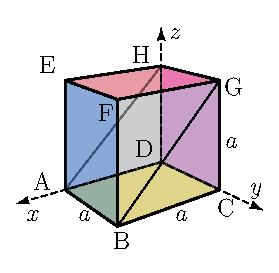
\includegraphics[scale=1]{figs/kocka_atloval.eps}
\caption{A kocka $BCGF$ és $ADHE$ lapátlóira, az $ABGH$ pontokra egy $n = \left( {1,0,1} \right)/\sqrt 2 $ normálisú síklapot fektetünk. }
\label{fig:kocka_atloval}
\end{figure}
\FloatBarrier

\paragraph{Megoldás}
\begin{enumerate}
\item 
Az egyensúly feltétele, hogy minden pontban az erők eredője 0. A kocka belsejében ez azt jelenti, hogy
\[\nabla {\mathbf{\sigma }} + \varrho {\mathbf{g}} = 0.\]
Kiírva a feszültségtenzor divergenciájának a definícióját kapjuk, hogy
\[\nabla {\mathbf{\sigma }} = \left( {\begin{array}{*{20}{c}}
  {{\partial _x}}&{{\partial _y}}&{{\partial _z}} 
\end{array}} \right)\left( {c\left( {\begin{array}{*{20}{c}}
  x&0&0 \\ 
  0&y&0 \\ 
  0&0&z 
\end{array}} \right)} \right) = c \cdot \left( {\begin{array}{*{20}{c}}
  1&1&1 
\end{array}} \right).\]
Visszahelyettesítve az előző egyenletbe:
\[{\mathbf{g}} =  - c \cdot /\varrho  \cdot \left( {\begin{array}{*{20}{c}}
  1&1&1 
\end{array}} \right).\] 
Ez egy konstans, $F$-ből $D$-felé mutató tömegerő, nagysága $g =  - c/\varrho  \cdot \sqrt 3 $.
\item A kocka oldallapjaira ható erő a feszültségtenzorból számolható.
\begin{enumerate}
\item Az $ABFE$ oldallap normálisa ${{\mathbf{n}}_{ABFE}} = \left( {1,0,0} \right)$, a felületi erősűrűség 
\[{{\mathbf{f}}_{ABFE}}\left( {\mathbf{r}} \right) = {\left. {{\mathbf{\sigma }}\left( {\mathbf{r}} \right)} \right|_{ABFE}} \cdot {{\mathbf{n}}_{ABFE}} = c\left( {\begin{array}{*{20}{c}}
  a&0&0 \\ 
  0&y&0 \\ 
  0&0&z 
\end{array}} \right)\left( {\begin{array}{*{20}{c}}
  1 \\ 
  0 \\ 
  0 
\end{array}} \right) = ca\cdot \left( {\begin{array}{*{20}{c}}
  1 \\ 
  0 \\ 
  0 
\end{array}} \right).\]
A teljes oldallapra ható erő:
\[\begin{aligned}
  {{\mathbf{F}}_{ABFE}} &  = \int_{ABFE} {{{\left. {{\mathbf{\sigma }}\left( {\mathbf{r}} \right)} \right|}_{ABFE}}} d{\mathbf{A}} \\ 
   &  = \int_{ABFE} {\underbrace {{{\left. {{\mathbf{\sigma }}\left( {\mathbf{r}} \right)} \right|}_{ABFE}}{{\mathbf{n}}_{ABFE}}}_{{{\mathbf{f}}_{ABFE}}\left( {\mathbf{r}} \right)}} dA \\ 
   &  = \int_{ABFE} {ca\left( {\begin{array}{*{20}{c}}
  1 \\ 
  0 \\ 
  0 
\end{array}} \right)dA}  \\ 
   &  = \int\limits_0^a {\int\limits_0^a 1 dy} dz \cdot ca\left( {\begin{array}{*{20}{c}}
  1 \\ 
  0 \\ 
  0 
\end{array}} \right) \\ 
   &  = c{a^3}\left( {\begin{array}{*{20}{c}}
  1 \\ 
  0 \\ 
  0 
\end{array}} \right) \\ 
\end{aligned} \]

\item A $DCGH$ oldallapon a feszültségtenzor releváns, $1,1$ komponense 0, így ott az erősűrűség és az erő is 0.
\item A $BCGF$ oldalon az $ABFE$ oldalhoz hasonlóan megmtutatható, hogy 
\[{{\mathbf{f}}_{BCGF}} = ca \cdot \left( {\begin{array}{*{20}{c}}
  0 \\ 
  1 \\ 
  0 
\end{array}} \right).\]
\item Az $ADHE$ oldalon a feszültségtenzor $2,2$ komponense 0, így ott a $DCGH$-hoz hasonlóan 0 az erősűrűség és az erő is.
\item Az $EFGH$ oldalon az $ABFE$ oldalhoz hasonlóan megmtutatható, hogy 
\[{{\mathbf{f}}_{EFGH}} = ca \cdot \left( {\begin{array}{*{20}{c}}
  0 \\ 
  0 \\ 
  1 
\end{array}} \right).\]
\item Az $ABCD$ oldalon a feszültségtenzor $3,3$ komponense 0, így ott a $DCGH$ oldalhoz hasonlóan 0 az erősűrűség és az erő is.
\end{enumerate}
\item Az $ABGH$ síkot olyan helyvektorok alkotják, amelyekre \[ABGH = \left\{ {{\mathbf{r}} = \left( {\begin{array}{*{20}{c}}
  x \\ 
  y \\ 
  z 
\end{array}} \right)|x + z = a;\;y} \right\}.\]
Erre a pontokra kell kiintegrálni ${\mathbf{\sigma }}$-t.
\[\begin{aligned}
  {{\mathbf{F}}_{ABGH}} &  = \int_{ABGH} {{{\left. {{\mathbf{\sigma }}\left( {\mathbf{r}} \right)} \right|}_{ABGH}}} d{\mathbf{A}} \\ 
   &  = \int_{ABGH} {c \cdot \left( {\begin{array}{*{20}{c}}
  x&0&0 \\ 
  0&y&0 \\ 
  0&0&{a - x} 
\end{array}} \right)} \left( {\begin{array}{*{20}{c}}
  1 \\ 
  0 \\ 
  1 
\end{array}} \right)/\sqrt 2 dA \\ 
   &  = \frac{c}{{\sqrt 2 }}\int_{ABGH} {\left( {\begin{array}{*{20}{c}}
  x \\ 
  0 \\ 
  {a - x} 
\end{array}} \right)} dA \\ 
   &  = \frac{c}{{\sqrt 2 }}\int\limits_0^a {\int\limits_0^a {\left( {\begin{array}{*{20}{c}}
  x \\ 
  0 \\ 
  {a - x} 
\end{array}} \right)} dx\sqrt 2  \cdot } dy \\ 
   &  = ca\int\limits_0^a {\left( {\begin{array}{*{20}{c}}
  x \\ 
  0 \\ 
  {a - x} 
\end{array}} \right)} dx \\ 
   &  = ca \cdot \frac{{{a^2}}}{2}\left( {\begin{array}{*{20}{c}}
  1 \\ 
  0 \\ 
  1 
\end{array}} \right) \\ 
   &  = \frac{{c{a^3}}}{2}\left( {\begin{array}{*{20}{c}}
  1 \\ 
  0 \\ 
  1 
\end{array}} \right) \\ 
\end{aligned} \]
Az integrál értékét meg is érezhetjük \aref{fig:ferde_int}.\ ábra alapján.
\begin{figure}[htb] 
\centering    
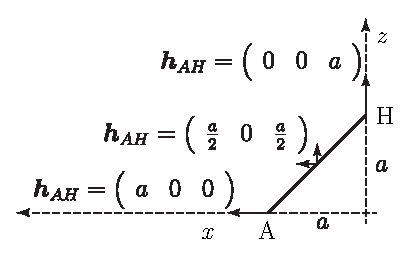
\includegraphics[scale=1]{figs/ferde_int.eps}
\caption{Az átló mentén a hossz szerint kell integrálnunk egy vektor mennyiséget, amelynek komponensei úgy függenek mind az $x$, mind a $z$ tengelytől, hogy összegük állandó.}
\label{fig:ferde_int}
\end{figure}
\FloatBarrier
\end{enumerate}
\normalsize

\subsection{Lehajlás}
Az előadáson bemutatták, hogyan hajlik le egy súlytalan rúd, amit egyik oldalán vízszintesen befognak, a másik, szabad oldalára pedig súlyt akasztanak.

A lehajlás vizsgálata során felírjuk a lehajló merev test egy kis részére az erőket azzal a közelítéssel, hogy a lehajlás a hosszhoz képest másodrendben kicsi, a rúd függőlegessel bezárt szögének koszinusza továbbra is 1 (azaz merőleges a függőlegesre), így az erők vízszintes vetületének kifejezéséhez nem kell figyelembe venni a lehajlást. A számolás során felhasználjuk, hogy a kicsiny darabra ható erők és forgatónyomatékok eredője 0. Az erőkre vonatkozó feltételből adódik a neutrális zóna helye, vagyis azon pontok helye, ahol 0 a deformáció. A forgatónyomatékra vonatkozó feltételben pedig megjelenik a 
\begin{equation} \label{eq:masodrendu_nyomatek}
{I_\Omega } = \int_\Omega  {{\xi ^2}dA}
\end{equation}
mennyiség, amelynek a neve \textbf{másodrendű nyomaték}, amelyben a $\xi$ a neutrális zónától vett távolság, az integrálást pedig arra a keresztmetszetre kell felírni, ami a merev test kis részét határolja.

Az egyik végén vízszintesen befogott rúd, amelynek szabad végére $F$ erő hat lefelé, $\Delta y$-nyit lehajlik, mégpedig a
\[\Delta y =  - \frac{F}{{EI}}\frac{{{l^3}}}{3}\]
összefüggés szerint, amelyben $E$ a Young-modulusz, $I$ a rúdra jellemző másodrendű nyomaték, $l$ pedig a rúd hossza.

\footnotesize
\paragraph{Példa}
Négyzet keresztmetszetű gerenda lehajlásához határozzuk meg a másodrendű nyomatékát, ha az oldalak függőleges és vízszintesek, illetve ha azzal $45^\circ$-os szöget zárnak be! Mekkora a másodrendű nyomatékok aránya?
\paragraph{Megoldás}
A neutrális zóna a négyzet közepén megy át, párhuzamosan az $x$ tengellyel. A másodrendű nyomatékot a
\[{I_\Omega } = \int_{\left[ { - a/2,a/2} \right] \times \left[ { - a/2,a/2} \right]} {{y^2}dA} \]
összefüggés adja. A 2D-s integrált felbontjuk 2 db 1D-s integrálra,
\[{I_\Omega } = \int\limits_{ - a/2}^{a/2} {\int\limits_{ - a/2}^{a/2} {{y^2}dx} dy} .\]
Az integrandus $x$-től független, ezért
\[{I_\Omega } = \int\limits_{ - a/2}^{a/2} {a{y^2}dy} .\]
Kiintegrálva a polinomot kapjuk, hogy 
\[{I_\Omega } = a\left. {\frac{1}{3}{y^3}} \right|_{ - a/2}^{a/2} = a\frac{1}{3}\left( {\frac{{{a^3}}}{8} - \frac{{ - {a^3}}}{8}} \right) = a\frac{1}{3}\frac{1}{4}{a^3} = \frac{{{a^4}}}{{12}}.\]

Elforgatott négyzet esetén a neutrális zóna a négyzet átlójában fut át. Bontsuk fel a négyzetet 4 db egybevágó derékszögű háromszögre, amelyek egyik befogója az $x$ tengelyen van, és végezzük el az integrálást csak erre arra az $\Omega_4$ tartományra, amelyet a bal alsó háromszög meghatároz! Az integrál értéke a négy háromszögön mind ugyanazt adják, így
\[{I_\Omega } = 4{I_{{\Omega _4}}} = 4\int_{{\Omega _4}} {{y^2}dA}.\]
A négyzet átlójának hossza $a\sqrt 2 $, így $x$-ben az integrál tartománya $\left[ { - a\sqrt 2 ,0} \right]$. Az $y$-ban vett integrálási tartomány felső határa a 0, az alsóé pedig $x$ értékétől függ, $y =  - x - a\sqrt 2 $. Kiírva az integrált:
\[{I_\Omega } = 4\int\limits_{ - a\sqrt 2 }^0 {\int\limits_{ - x - a\sqrt 2 }^0 {{y^2}} dy} dx.\]
A belső integrandus $x$-től független, így az integrál értéke
\[{I_\Omega } = 4\int\limits_{ - a\sqrt 2 }^0 {\left. {\frac{1}{3}{y^3}} \right|_{ - x - a\sqrt 2 }^0} dx = 4\frac{1}{3}\int\limits_{ - a\sqrt 2 }^0 {0 - {{\left( { - x - a\sqrt 2 } \right)}^3}} dx = \frac{4}{3}\int\limits_{ - a\sqrt 2 }^0 {{{\left( {x + a\sqrt 2 } \right)}^3}dx} .\]
Nem bontjuk ki a zárójelet csak azért, hogy tagonként integrálhassunk, hanem beírjuk egyből ${\left( {x + c} \right)^n}$ integrálját, hiszen ezt deriválni is könnyű, így nagy kő esik le a szívünkről:
\[{I_\Omega } = \frac{4}{3} \cdot \left. {\frac{1}{4}{{\left( {x + a\sqrt 2 /2} \right)}^4}} \right|_{ - a\sqrt 2 /2}^0 = \frac{4}{3}\frac{1}{4}\frac{{{a^4}}}{4} = \frac{{{a^4}}}{{12}}.\]
Meglepődve láthatjuk, hogy ez ugyanannyi, mint az előbbi eseté. Ez csak azért van így, mert négyzetet néztünk, téglalapra nem így lett volna. Egy négyzetet vajon $30^\circ$-kal elforgatva is ugyanezt kaptuk volna? És mi a helyzet tetszőleges szög esetére? Megannyi kínzó kérdés!

\paragraph{Példa}
Mekkora egy üreges négyzetes hasábra a másodrendű nyomaték, ha a külső oldalél $a_k$ hosszúságú, a belső üreg oldaléle pedig $a_b$?
\paragraph{Megoldás}
Felbonthatnánk az integrálást ismét 4 tartományra, és összeadhatnánk azok másodrendű nyomatékát, majd az integrálási határokat ügyesen kijelölve, vagy a tartományokat átdarabolva elvégezhetnénk az integrálást. Egyszerűbb azonban, ha a nagy négyzet másodrendű nyomatékából kivonjuk a kis négyzet másodrendű nyomatékát. Tehetjük mindezt azért, mert
\[{I_{{\Omega _t}}} = {I_\Omega } + {I_{{\Omega _b}}} \Rightarrow \int_{{\Omega _t}}  \ldots   = \int_\Omega   \ldots   + \int_{{\Omega _b}}  \ldots ,\]
ahol ${\Omega _t}$ a tömör, teljes négyzet tartománya, $\Omega$ az üreges négyzet tartománya, $\Omega_b$ pedig a belső, üreges rész tartománya. Így a keresett $I_\Omega$ értékére kapjuk, hogy
\[{I_\Omega } = \frac{{a_k^4 - a_b^4}}{{12}}.\]

\paragraph{Példa}
Négyzet keresztmetszetű, $5{\text{ mm}}$ oldalélű vas ruhaakasztóként szolgál, hossza $5{\text cm}$. Mekkora lehet a végére akasztott legnagyobb tömegű kabát, hogy a lehajlása még ne érje el az $1{\text{ mm}}$-t? A vas Young-modulusza $100{\text{ GPa}}$, a négyzet másodrendű nyomatéka $I = {a^4}/12$, ahol $a$ a négyzet oldalának a hossza.
\paragraph{Megoldás}
\[\Delta y =  - \frac{F}{{EI}}\frac{{{l^3}}}{3} \Rightarrow F =  - \frac{{3EI\Delta y}}{{{l^3}}} =  - \frac{{3 \cdot 200 \cdot {{10}^9} \cdot \frac{1}{{12}}{{\left( {5 \cdot {{10}^{ - 3}}} \right)}^4} \cdot 1 \cdot {{10}^{ - 3}}}}{{{{\left( {5 \cdot {{10}^{ - 2}}} \right)}^3}}}{\text{ N}} =  - 250{\text{ N}}\]
Vagyis kb.\ $25 {\text{ kg}}$-nyi súlyt akaszthatunk a fogas végére.
\normalsize

\section{Hidrosztatika}
Olyan eseteket nézünk, ahol a közeg folyadék vagy gáz, és a sebességtér konstans 0. Ekkor a feszültségtenzor csak az egységmátrixszal lehet arányos.

A nyomás, sűrűség és erőpotenciál kapcsolatát a 
\[{\text{grad}}\left( {p\left( {\mathbf{r}} \right)} \right) =  - \rho \left( {\mathbf{r}} \right) \cdot {\text{grad}}\left( {\phi \left( {\mathbf{r}} \right)} \right)\]
összefüggés adja meg. Ha a sűrűség térben állandó és a potenciált az homogén gravitációs térből számoljuk, akkor a nyomás a mélységgel lineárisan nő és
\[p = {p_0} + \rho gh.\]

A felhajtóerő minden közegben lévő testre hat, és amennyiben a közeg a testet minden oldalról körülveszi, és ha a közeg sűrűsége a test méretének tartományában állandó, az értéke
\[{{\mathbf{F}}_f} =  - {\rho _{{\text{közeg}}}}{\mathbf{g}}V.\]

Ha a nyomás és a sűrűség egymással arányos (mint pl.\ ideális gázoknál), akkor homogén gravitációs térben a nyomás felfelé exponenciálisan csökken és
\[\rho \left( z \right) = {\rho _0} \cdot {e^{\frac{{ - mgz}}{{{k_B}T}}}}.\]
\footnotesize
\paragraph{Példa}
A Balaton partján felfújunk egy leeresztve $10 \text{ kg}$ tömegű gumicsónakot, aminek így a térfogata $0{,}7\text{ m}^3$ lesz (kezdeti térfogata elhanyagolható), benne a nyomás $110\text{ kPa}$, míg a légköri nyomás $100\text{ kPa}$. A levegő sűrűsége légköri nyomáson, a fújáskori hőmérsékleten $1{,}2\text{ kg}/\text{m}^3$ (a hőmérséklet a csónakon kívül és belül megegyezik).

Mekkora a gumicsónak össztömege? Mekkora a súlya? Mennyivel kisebb tömegű az a csónak, aminek súlyának ez megfelel? Legfeljebb mekkora hasznos tömeget szállíthat a csónak a saját tömegén felül? A víz sűrűségét tekintsük $1000\text{ kg}/\text{m}^3$-nek, a nehézségi gyorsulás értékét $10\text{ m}/\text{s}^2$-nek!

\paragraph{Megoldás}
A csónak tömege a belefújt levegőével növekszik. A csónakon belüli és kívüli hőmérséklet azonos, így
\[pV = nRT = \frac{m}{M}RT \Rightarrow \frac{p}{\varrho } = {\text{állandó}}.\]
Így a csónakon belüli sűrűség a benti és kinti nyomások arányával egyezik meg,
\[{\varrho _{{\text{bent}}}} = {\varrho _{{\text{kint}}}} \cdot \frac{{110}}{{100}}.\]
A felfújt csónak teljes tömege így
\[{m_{{\text{teljes}}}} = {m_\text{csónak}} + {m_\text{levegő}} = \left( {10 + \underbrace {1{,}2 \cdot \frac{{110}}{{100}}}_{{\varrho _{{\text{bent}}}}} \cdot \underbrace {0{,}7}_V} \right){\text{ kg}} = 10{,}924{\text{ kg}}.\]
A csónak tömege tehát majdnem $9\%$-kal növekedett. A csónak súlya a kiszorított $0{,}7\text{ m}^3$ levegő súlyával csökken ahhoz képest, mintha nem lenne légkör,
\[F = {m_\text{teljes}} \cdot g - V \cdot {\varrho _\text{levegő}}g = \left( {{m_\text{teljes}} - V \cdot {\varrho _\text{levegő}}} \right)g \approx \left( {10{,}924 - 0{,}7 \cdot 1{,}2} \right)10{\text{ N}} = 100{,}84{\text{ N}}.\]
Ez csak közel $1\%$-kal nagyobb, mint a csónak eredeti súlya. A súly növekedését kifejezhetjük a többletnyomásból származó többletsúllyal is,
\[F = m_\text{csónak}g + 1{,}2 \cdot \frac{{10}}{{100}}0{,}7 \cdot 10{\text{ N}} = \left( {100 + 0{,}84} \right){\text{ N}} = 100{,}84{\text{ N}}.\]
A csónakot annyival érezzük könnyebnek a tömege alapján indokolt súlynál, mint amennyi a légkörből kiszorított levegő súlyának megfelelő tömeg,
\[\Delta m = V \cdot {\varrho _\text{levegő}} = {\text{0{,}84 kg}},\]
vagyis ekkora tömegnek megfelelő súllyal érezzük a csónakot könnyebnek, ha a csónak tartásáról, azaz a súlyáról van szó. A gyorsításához továbbra is a teljes tömegét kell figyelembe venni. A csónakra ható felhajtóerő elméleti maximuma a kiszorított $0{,}7\text{ m}^3$ térfogatú víz súlya lehet,
\[F = V \cdot \varrho  \cdot g = 0,7 \cdot 1000 \cdot 10{\text{ N}} = 7000{\text{ N}}.\]
Az ekkora súlyhoz tartozó tömeg $700\text{ kg}$, amelyből $10{,}924{\text{ kg}}$ a csónak saját, teljes tömege, így legfeljebb $\left( {700 - 10,924} \right){\text{ kg}} \approx 689{\text{ kg}}$ tömeget tud szállítani.

\paragraph{Példa}
Egy érzékeny kétkarú mérleg egyik serpenyőjébe egy nagy, vízzel félig telt főzőpoharat teszünk, majd másik oldalon súlyokkal kiegyensúlyozzuk. Mit mutat a mérleg, ha a főzőpohárban lévő vízbe -- a pohárhoz való hozzáérés nélkül -- lógatunk egy testet, aminek a sűrűsége a víznél
\begin{enumerate}
\item kisebb,
\item megegyező,
\item nagyobb?
\end{enumerate}

\paragraph{Megoldás}
Ahelyett, hogy a pohár -- víz alkotta rendszert vizsgáljuk, és a rá ható erők eredőjét nézzük, tekintsük csak a poharat és a rá ható erőket! A pohár egyensúlyban van, így a rá ható erők összege 0. Hat rá a nehézségi erő, a folyadék valamilyen átlagos ${\mathbf{\sigma }} =  - p{\mathbf{ I}}$ nyomásából származó, valamilyen $A$ effektív felületen kifejtett erőből, illetve a mérleg serpenyője által kifejtett tartóerőből.
\[F = mg + A \cdot p + {F_{{\text{tart}}}},\]
amelyben
\[p = {\varrho _{{\text{viz}}}}gh.\]
Ha most bármilyen sűrűségű testet a vízbe lógatunk, akkor a vízszint megemelkedik, miközben adott minden $h$ mélységben a nyomás továbbra is a fenti képlet szerint számolható. Így a pohár alján a nyomás is megnövekedik, ezért nagyobb ellenerőt kell kifejtenie a mérleg karjának, tehát a vizes poharas serpenyőt jelzi nehezebbnek.

Ugyanerre jutunk, ha a pohár vízzel + test egyensúlyát nézzük. Ekkor azt jó figyelni, hogy a rendszer egyensúlyához a rá ható nehézségi erő ellensúlyozására nemcsak a serpenyő tartóerőerje járul hozzá, hanem a mi általunk kifejtett tartóerő (ami mint felfüggesztés húzza a testet). Amikor a test nem lóg bele a vízbe, mi kifejtünk valamekkora erőt. Amikor már belelóg, akkor mi kisebbet fejtünk ki, mint korábban. (Ha a test lebegni tud a vizen, akkor az általunk kifejtett akár 0-ig is csökkenhet.) Tekintve, hogy a nehézségi erő ellen ható tartóerőnk csökken, az erők egyensúlya csak úgy valósulhat meg, ha a tálca nagyobb erőt fejt ki, vagyis a mutató ismét kitért, a poharas serpenyőt jelzi nehezebbnek.

\paragraph{Példa}
Egy csonkakúp-alakú test a szimmetriatengelyével függőlegesen úgy úszik egy higanyt tartalmazó edényben, hogy térfogatának negyede merül a higanyba.
\begin{enumerate}
\item A magyar helyesírás szabályainak megfelele-e a "csonkakúp-alakú" kifejezés?
\item Mekkora része merülne a higanyaba a testnek, ha annyi vizet töltenénk az  edénybe, hogy az elfedje a csonka kúpot?
\end{enumerate}

\paragraph{Megoldás}
\begin{enumerate}
\item Ha a Magyar Helyesírás Szabályai, 141.b) az irányadó, akkor igen. Eszerint:

"Ha egy különírt szókapcsolat (pl. hajlított bútor) olyan utótagot kap (pl. gyár), amely az egész kapcsolathoz járul, az egyébként különírandó részt az új alakulatban egybeírjuk, és ehhez az utótagot (a szótagszámtól függetlenül) kötőjellel kapcsoljuk: hajlítottbútor-gyár. Hasonló esetek: hideg víz, de: hidegvíz-csap; házi feladat, de: házifeladat-készítés; légi fénykép, de: légifénykép-montázs; stb\ldots"

Egy másik vélemény szerint nem, mert \ldots
\item Számoljuk ki a sűrűségét az alapján, hogy negyedig merül el a higanyban. Ez biztos hasznos lesz.
\[F = 0 = \underbrace {g{\varrho _{Hg}}\frac{{{V_{{\text{csk}}}}}}{4}}_{{\text{felhatjóerő}}} - \underbrace {g{\varrho _{{\text{csk}}}}{V_{{\text{csk}}}}}_{{\text{súlyerő}}} \Rightarrow {\varrho _{{\text{csk}}}} = \frac{{{\varrho _{Hg}}}}{4}\]
Miután vizet töltünk rá, higany és víz veszi körül (nem keverednek), de csak valamilyen mértében van egyikben, és másikban elmerülve: legyen $\alpha$ mértékben elmerülve a higanyban! Amit tudunk még, hogy a kiszorított térfogatok összege $V$, és a rá ható erők eredője.
\[F = 0 = \underbrace {g{\varrho _{Hg}}\cdot{V_{{\text{csk}}}} \alpha }_{Hg{\text{ felhajtóerő}}} + \underbrace {g{\varrho _{{\text{víz}}}}\cdot{V_{{\text{csk}}}} \left( {1 - \alpha } \right)}_{{\text{víz felhajtóerő}}} - \underbrace {g\frac{{{\varrho _{Hg}}}}{4}{V_{{\text{csk}}}}}_{{\text{súlyerő}}}\]
Ez egy egyenlet $\alpha$-ra, más ismeretlen nincs benne.

\[\begin{gathered}
  {\varrho _{Hg}} \cdot \alpha  + {\varrho _{{\text{viz}}}} - {\varrho _{{\text{viz}}}}\alpha  - {\varrho _{Hg}}/4 = 0 \hfill \\
  \alpha  = \frac{{{\varrho _{Hg}}/4 - {\varrho _{{\text{viz}}}}}}{{{\varrho _{Hg}} - {\varrho _{{\text{viz}}}}}} \approx \frac{{14/4 - 1}}{{14 - 1}} \approx 0,2 \hfill \\ 
\end{gathered} \]
\end{enumerate}

\paragraph{Példa}
Egy üvegkádra kerekeket szerelünk, vizet töltünk bele, egy lejtőre tesszük, és miután a lejtés irányába beirányítjuk, elengedjük.
\begin{itemize}
\item  Egyensúlyban mekkora szöget zár be a kádban a víz felszíne a kád oldalával, ha a lejtő nyílásszöge $\alpha$ és a súrlódástól eltekintünk?
\item A kád fenekén hol mekkora a víztől származó nyomás, ha a kád vízszintes helyzetében a víz a kád oldalán $l$ magasságig ért?
\end{itemize}

\paragraph{Megoldás}
A jelenség leírási egyszerű a káddal együtt mozgó koordináta-rendszerben. Ebben a rendszerben a kád és a vele együtt a folyadék is nyugalomban van. A folyadék felszíne a folyadékrészekre ható erők eredőjére merőleges, ugyanis az ekvipotenciális felületeken az adott pontban ható erő a felületre mindig merőleges. Gyorsuló rendszerben történő leírásnál a tényleges erőkön felül a tehetetlenségi erőket is figyelembe kell venni. A jelenséget úgy írjuk le, hogy az $m$ tömegű folyadékrészre a függőleges irányú $mg$ nehézségi erőn felül a lejtővel párhuzamos és az emelkedés felé mutató, $ma$ nagyságú tehetetlenségi erő is hat, amelyben a gyorsulást a nehézségi erő lejtő irányú komponense adja.

\begin{figure}[htb] 
\begin{subfigure}[b]{0.45\textwidth}
\centering
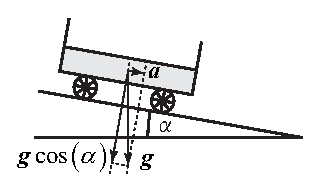
\includegraphics[scale=1]{figs/uvegkad_a.eps}
\caption{A lejtőn guruló üvegkád ${\mathbf{a}}$ gyorsulásának a nagysága $a = g \cdot \sin \left( \alpha \right)$, amit az álló vonatkoztatási rendszerből írhatunk fel, mint a nehézségi gyorsulás lejtő irányú vetülete. Inerciarendszerben nem hatnak tehetetlenségi erők.}
\end{subfigure}
\begin{subfigure}[b]{0.45\textwidth}
\centering
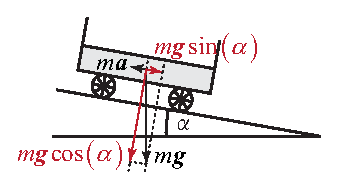
\includegraphics[scale=1]{figs/uvegkad_b.eps}
\caption{A gyorsuló rendszerben ható erők (fekete), illetve a nehézségi erő felbontása (piros). A nehézségi erő lejtő irányú komponensét a tehetetlenségi erő kioltja, csak a nehézségi erő lejtőre merőleges komponense marad.}
\end{subfigure}
\label{fig:uvegkad}
\end{figure}
\FloatBarrier

\begin{itemize}
\item Felbontva a nehézségi erőt lejtő irányú, és arra merőleges komponensre, a lejtő irányú komponenst a tehetetlenségi erő épp kioltja. Tehát az eredő erő a gyorsuló vonatkoztatási rendszerben lejtőre merőleges irányú. A gravitációs és tehetetlenségi erőkhöz tartozó ekvipotenciálos felületek tehát a lejtővel párhuzamosak, így a folyadék felszíne is párhuzamos a lejtővel. 
\item Egy kis $m$ tömegű folyadékrészre összesen a lejtőre merőleges irányú és $mg \cdot \cos \left( \alpha  \right)$ nagyságú erő hat. Ebből következően a nyomás az edény fenekén mindenhol állandó nagyságú és értéke $mgl \cdot \cos \left( \alpha  \right)$, vagyis $\cos \left( \alpha  \right)$ szorosa annak, mintha a kád nyugalomban állna egy vízszintes talajon.
\end{itemize}

\paragraph{Példa}
Függőleges falú, vízzel töltött medencében kővel terhelt csónak úszik a vízen. Változik-e a medencében a víz szintjének a magassága, ha a köveket a csónakból a vízbe dobjuk?

\paragraph{Megoldás}
Legyen a medence aljának területe $A$, a vízszint magassága (mikor a terhelt csónak úszik rajta) $h_1$, a kövek vízbedobása után pedig $h_2$! Legyen az üres csónak súlya $G_1$, a köveké pedig $G$! A terhelt csónak által kiszorított víz térfogata $V_1$, az üres csónak által kiszorított víz térfogata $V_1$, a medencében lévő víz térfogata pedig $V$! Ekkor
A kővel terhelt és nem terhelt csónak is úszik a víz felszínén, ezért
\[{G_1} + G = {\varrho _{\text{víz}}}{V_1}g,\]
illetve
\[G = {\varrho _{\text{víz}}}{V_2}g.\]
Ebből
\[{V_1} - {V_2} = \frac{G}{{g{\varrho _{\text{víz}}}}} = \frac{{{\varrho _{\text{kő}}}{V_{\text{kő}}}}}{{{\varrho _{\text{víz}}}}}.\]
A medence aljától a víz felszínéig tartó részének a térfogatára (ha a kő elsüllyed a vízben):
\[\begin{aligned}
  A{h_1} =  & V + {V_1}, \\ 
  A{h_2} =  & V + {V_{{\text{kő}}}} + {V_2}, \\ 
\end{aligned} \]
amelyből
\[A\left( {{h_1} - {h_2}} \right) = {V_1} - {V_2} - {V_{{\text{kő}}}} = {V_{{\text{kő}}}}\left( {\frac{{{\varrho _{{\text{kő}}}}}}{{{\varrho _{{\text{víz}}}}}} - 1} \right),\]
így a magasságkülönbségre adódik, hogy
\[{h_1} - {h_2} = \frac{1}{A}{V_{{\text{kő}}}}\left( {\frac{{{\varrho _{{\text{kő}}}} - {\varrho _{{\text{víz}}}}}}{{{\varrho _{{\text{víz}}}}}}} \right).\]
Ha tehát a kő sűrűsége nagyobb, mint a vízé, akkor $h_1 > h_2$, vagyis a víz magassága a kövek bedobálásával csökken. (Ha a kő sűrűsége kisebb, mint a vízé, akkor a kő úszna a vízfelszínen, és nem süllyedne el, amit feltettünk. Végigszámolva ezt az esetet azt kapnánk, hogy a vízszint nem változna.)
\normalsize

\section{Felületi feszültség}
A felületi feszültség nyugvó gáz és folyadék, illetve szilárd anyagra bevezetett fogalom, ahol két különféle halmazállapotú anyag (akár azonos halmazállapotból véve) közötti határfelületet vizsgáljuk. Általában nem vizsgálunk szilárd anyag-szilárd anyag határfelületet, mert közöttük a feszültségtenzor nyíró komponenst is tartalmazhat, tehát azok az egységmátrixnak nem skalárszorosai, így esetükben nyomásról nem beszélhetünk.

Egy $l$ hosszúságú szakaszra a közeg határán
\[F = 2\alpha  \cdot l\]
nagyságú erő hat, és a felület csökkenésének irányába mutat.

A felületi feszültség következményeként minden közeghatárhoz tartozik egy felületi energia, amely arányos a felület nagyságával és 
\[E = \alpha A.\]

Egy kellően kicsiny, $R_1$ és $R_2$ görbületi sugárral jellemzett konvex (nem nyeregponti) felület belső oldalán $p_g$ többletnyomás szükséges az egyensúlyhoz, ahol
\[{p_g} = \alpha \left( {\frac{1}{{{R_1}}} + \frac{1}{{{R_2}}}} \right)\]
a görbületi nyomás. Ha a felület gömbhéj, akkor $R_1 = R_2$.
\footnotesize
\paragraph{Példa}
Mennyi munkára van szükség ahhoz, hogy egy $2\text{ mm}$ sugarú higanycseppet (felületi feszültség $0{,}52\text{ N}/\text{m}$) két egyforma méretű higanycseppé vágjuk szét?

\paragraph{Megoldás}
A nagy higanycsepp indexe legyen az 1-es, a két kicsihez tartozó a 2-es. A két esetben a térfogat megegyezik.
\[\begin{aligned}
  {V_1} &  = {V_2} \\ 
  \frac{4}{3}r_1^3\pi  &  = 2 \cdot \frac{4}{3}r_2^3\pi  \Rightarrow {r_2} = {2^{ - \frac{1}{3}}}{r_1} \\ 
\end{aligned} \]
A felületek nem egyeznek meg, a növekedést akarjuk kiszámolni.
\[\begin{gathered}
  {A_1} = 4r_1^2\pi  \hfill \\
  {A_2} = 2 \cdot 4r_2^2\pi  = 2 \cdot 4 \cdot {\left( {{2^{ - \frac{1}{3}}}} \right)^2}r_1^2\pi  = {2^{\frac{1}{3}}}{A_1} \Rightarrow \Delta A = \left( {{2^{\frac{1}{3}}} - 1} \right)4r_1^2\pi  \hfill \\ 
\end{gathered} \]
Az energia-változást ebből már kifejezhetjük.
\[W = \Delta A \cdot \alpha  = \left( {{2^{\frac{1}{3}}} - 1} \right)4r_1^2\pi  \cdot \alpha  = \left( {{2^{\frac{1}{3}}} - 1} \right)4 \cdot {2^2} \cdot {10^{ - 6}}\pi  \cdot 0{,}52{\text{ J}} \approx {\text{6{,}8}} \cdot {\text{1}}{{\text{0}}^{ - 6}}{\text{ J}}\]
\paragraph{Példa}
A szappan-levegő felületi feszültsége $\alpha = 0{,}025\text{ N}/\text{m}$. 
\begin{enumerate}
\item  Milyen méretű buborék esetén lenne a nyomás kétszerese a légköri nyomásnak? 
\item Hány százalékkal nagyobb a nyomás egy $1\text{ mm}$ átmérőjű szappanbuborékban, mint a körülötte lévő légköri levegőben, ahol a nyomás $10^5\text{ Pa}$?
\item Mekkorára fújódna fel a buborék, ha a légköri nyomás megszűnne, de a buborék nem pukkadna ki?
\end{enumerate}

\paragraph{Megoldás}
A görbületi nyomás formulája
\[{p_g} = \alpha \left( {\frac{1}{R} + \frac{1}{R}} \right).\]
\begin{enumerate}
\item A görbületi nyomás szolgáltasson egy extra légköri nyomásnyit!
\[R = \frac{{2\alpha }}{p_g} = 2 \cdot \frac{{0{,}025}}{{{{10}^5}}}{\text{m}} = 5 \cdot {10^{ - 7}}{\text{ m}} = 500{\text{ nm}}\]
Ez a fény hullámhosszának nagyságrendjébe esik.
\item A többletnyomás a képletbe való behelyettesítéssel:
\[{p_g} = 0{,}025\frac{2}{{{{10}^{ - 3}}/2}}{\text{Pa}} = 100{\text{ Pa}}.\]
Ez a légköri nyomás $0{,}1\%$-a.
\item Bal oldalt a légköri nyomás mellett, jobb oldalt a légköri nyomás nélkül a buborékban lévő levegőre vonatkoztatott értékek, 
\[\begin{aligned}
  {p_1}{V_1} &  = {p_2}{V_2} \\ 
  \left( {{p_0} + \frac{{2\alpha }}{R}} \right)\frac{4}{3}{R^3}\pi  &  = \frac{{2\alpha }}{{R'}} \cdot \frac{4}{3}R{'^3}\pi  \Rightarrow R' = \sqrt {\frac{{{p_0}R}}{{2\alpha }} + 1}  \cdot R. \\ 
\end{aligned} \]
Behelyettesítés után adódik, hogy $R' = 44{,}7{\text{ mm}}$.
\end{enumerate}
\normalsize
\end{document}

